\documentclass[12pt,]{book}
\usepackage{lmodern}
\usepackage{amssymb,amsmath}
\usepackage{ifxetex,ifluatex}
\usepackage{fixltx2e} % provides \textsubscript
\ifnum 0\ifxetex 1\fi\ifluatex 1\fi=0 % if pdftex
  \usepackage[T1]{fontenc}
  \usepackage[utf8]{inputenc}
\else % if luatex or xelatex
  \ifxetex
    \usepackage{mathspec}
  \else
    \usepackage{fontspec}
  \fi
  \defaultfontfeatures{Ligatures=TeX,Scale=MatchLowercase}
    \setmonofont[Mapping=tex-ansi,Scale=0.7]{Source Code Pro}
\fi
% use upquote if available, for straight quotes in verbatim environments
\IfFileExists{upquote.sty}{\usepackage{upquote}}{}
% use microtype if available
\IfFileExists{microtype.sty}{%
\usepackage{microtype}
\UseMicrotypeSet[protrusion]{basicmath} % disable protrusion for tt fonts
}{}
\usepackage[margin=1in]{geometry}
\usepackage{hyperref}
\hypersetup{unicode=true,
            pdftitle={The Sainsbury Laboratory Summer School 2017},
            pdfborder={0 0 0},
            breaklinks=true}
\urlstyle{same}  % don't use monospace font for urls
\usepackage{natbib}
\bibliographystyle{apalike}
\usepackage{longtable,booktabs}
\usepackage{graphicx,grffile}
\makeatletter
\def\maxwidth{\ifdim\Gin@nat@width>\linewidth\linewidth\else\Gin@nat@width\fi}
\def\maxheight{\ifdim\Gin@nat@height>\textheight\textheight\else\Gin@nat@height\fi}
\makeatother
% Scale images if necessary, so that they will not overflow the page
% margins by default, and it is still possible to overwrite the defaults
% using explicit options in \includegraphics[width, height, ...]{}
\setkeys{Gin}{width=\maxwidth,height=\maxheight,keepaspectratio}
\IfFileExists{parskip.sty}{%
\usepackage{parskip}
}{% else
\setlength{\parindent}{0pt}
\setlength{\parskip}{6pt plus 2pt minus 1pt}
}
\setlength{\emergencystretch}{3em}  % prevent overfull lines
\providecommand{\tightlist}{%
  \setlength{\itemsep}{0pt}\setlength{\parskip}{0pt}}
\setcounter{secnumdepth}{5}
% Redefines (sub)paragraphs to behave more like sections
\ifx\paragraph\undefined\else
\let\oldparagraph\paragraph
\renewcommand{\paragraph}[1]{\oldparagraph{#1}\mbox{}}
\fi
\ifx\subparagraph\undefined\else
\let\oldsubparagraph\subparagraph
\renewcommand{\subparagraph}[1]{\oldsubparagraph{#1}\mbox{}}
\fi

%%% Use protect on footnotes to avoid problems with footnotes in titles
\let\rmarkdownfootnote\footnote%
\def\footnote{\protect\rmarkdownfootnote}

%%% Change title format to be more compact
\usepackage{titling}

% Create subtitle command for use in maketitle
\newcommand{\subtitle}[1]{
  \posttitle{
    \begin{center}\large#1\end{center}
    }
}

\setlength{\droptitle}{-2em}
  \title{The Sainsbury Laboratory Summer School 2017}
  \pretitle{\vspace{\droptitle}\centering\huge}
  \posttitle{\par}
  \author{}
  \preauthor{}\postauthor{}
  \date{}
  \predate{}\postdate{}

\usepackage{booktabs}
\usepackage{amsthm}
\makeatletter
\def\thm@space@setup{%
  \thm@preskip=8pt plus 2pt minus 4pt
  \thm@postskip=\thm@preskip
}
\makeatother
\setmainfont[UprightFeatures={SmallCapsFont=AlegreyaSC-Regular}]{Alegreya}
\renewcommand{\textfraction}{0.05}
\renewcommand{\topfraction}{0.8}
\renewcommand{\bottomfraction}{0.8}
\renewcommand{\floatpagefraction}{0.75}
\let\oldhref\href
\renewcommand{\href}[2]{#2\footnote{\url{#1}}}

\begin{document}
\maketitle

{
\setcounter{tocdepth}{1}
\tableofcontents
}
\chapter*{Welcome to The Sainsbury Laboratory Summer School
2017}\label{welcome-to-the-sainsbury-laboratory-summer-school-2017}
\addcontentsline{toc}{chapter}{Welcome to The Sainsbury Laboratory
Summer School 2017}

The last 20 years have provided a sophisticated understanding of how
plants recognise relatively conserved microbial patterns to activate
defence. In recent years DNA sequencing has allowed genomes and
transcriptomes of eukaryotic rusts and mildew pathogens to be studied.
High-throughput imaging advances have made possible the study and
visualisation of intracellular interactions during pathogenesis and
defence.

We will present and teach on these many aspects of plant-microbe
interactions from the fundamental genomic, cellular and molecular
processes to translational activities about how we convert basic
discovery to real world impact.

The TSL Summer School will focus on dynamic and interactive practical
sessions will naturally promote strong interactions between speakers and
participants.

Over the next two weeks we will cover a wide range of topics, including:

\begin{itemize}
\tightlist
\item
  Pathogenomics
\item
  Effectors
\item
  Surface Immunity
\item
  Bioinformatics
\item
  Resistance Proteins
\item
  Cellular Defence
\item
  Proteomics
\item
  Wheat Genomics
\item
  Translation to the field
\end{itemize}

We hope that you will find the whole exercise enlightening and
educational and perhaps also a little fun.

\chapter*{Course schedule}\label{course-schedule}
\addcontentsline{toc}{chapter}{Course schedule}

\section*{Monday 31st July}\label{monday-31st-july}
\addcontentsline{toc}{section}{Monday 31st July}

\emph{Introductions}

\begin{longtable}[]{@{}lll@{}}
\toprule
\begin{minipage}[b]{0.09\columnwidth}\raggedright\strut
Time\strut
\end{minipage} & \begin{minipage}[b]{0.38\columnwidth}\raggedright\strut
Activity\strut
\end{minipage} & \begin{minipage}[b]{0.38\columnwidth}\raggedright\strut
Venue\strut
\end{minipage}\tabularnewline
\midrule
\endhead
\begin{minipage}[t]{0.09\columnwidth}\raggedright\strut
1000\strut
\end{minipage} & \begin{minipage}[t]{0.38\columnwidth}\raggedright\strut
Welcome to TSL and housekeeping\strut
\end{minipage} & \begin{minipage}[t]{0.38\columnwidth}\raggedright\strut
\strut
\end{minipage}\tabularnewline
\begin{minipage}[t]{0.09\columnwidth}\raggedright\strut
1015\strut
\end{minipage} & \begin{minipage}[t]{0.38\columnwidth}\raggedright\strut
Introductions by TSL Staff\strut
\end{minipage} & \begin{minipage}[t]{0.38\columnwidth}\raggedright\strut
\strut
\end{minipage}\tabularnewline
\begin{minipage}[t]{0.09\columnwidth}\raggedright\strut
1030\strut
\end{minipage} & \begin{minipage}[t]{0.38\columnwidth}\raggedright\strut
Participant Introductions\strut
\end{minipage} & \begin{minipage}[t]{0.38\columnwidth}\raggedright\strut
\strut
\end{minipage}\tabularnewline
\begin{minipage}[t]{0.09\columnwidth}\raggedright\strut
1100\strut
\end{minipage} & \begin{minipage}[t]{0.38\columnwidth}\raggedright\strut
PEDAGOGICAL LECTURE - Introduction to Plant Microbe Interactions\strut
\end{minipage} & \begin{minipage}[t]{0.38\columnwidth}\raggedright\strut
\strut
\end{minipage}\tabularnewline
\begin{minipage}[t]{0.09\columnwidth}\raggedright\strut
1200\strut
\end{minipage} & \begin{minipage}[t]{0.38\columnwidth}\raggedright\strut
Lunch\strut
\end{minipage} & \begin{minipage}[t]{0.38\columnwidth}\raggedright\strut
NRP Venues\strut
\end{minipage}\tabularnewline
\begin{minipage}[t]{0.09\columnwidth}\raggedright\strut
1300\strut
\end{minipage} & \begin{minipage}[t]{0.38\columnwidth}\raggedright\strut
Poster Session\strut
\end{minipage} & \begin{minipage}[t]{0.38\columnwidth}\raggedright\strut
John Innes Centre Conference Centre\strut
\end{minipage}\tabularnewline
\begin{minipage}[t]{0.09\columnwidth}\raggedright\strut
1500\strut
\end{minipage} & \begin{minipage}[t]{0.38\columnwidth}\raggedright\strut
Tour of The Sainsbury Laboratory and Norwich Research Park\strut
\end{minipage} & \begin{minipage}[t]{0.38\columnwidth}\raggedright\strut
Meet at John Innes Reception\strut
\end{minipage}\tabularnewline
\bottomrule
\end{longtable}

NB All activities will take place in the Training Suite, unless
otherwise stated

\section*{Tuesday 1st August}\label{tuesday-1st-august}
\addcontentsline{toc}{section}{Tuesday 1st August}

\emph{Resistance Proteins. Led by Jonathan Jones}

\begin{longtable}[]{@{}lll@{}}
\toprule
\begin{minipage}[b]{0.09\columnwidth}\raggedright\strut
Time\strut
\end{minipage} & \begin{minipage}[b]{0.39\columnwidth}\raggedright\strut
Activity\strut
\end{minipage} & \begin{minipage}[b]{0.39\columnwidth}\raggedright\strut
Venue\strut
\end{minipage}\tabularnewline
\midrule
\endhead
\begin{minipage}[t]{0.09\columnwidth}\raggedright\strut
930\strut
\end{minipage} & \begin{minipage}[t]{0.39\columnwidth}\raggedright\strut
PEDAGOGICAL LECTURE - Jonathan Jones\strut
\end{minipage} & \begin{minipage}[t]{0.39\columnwidth}\raggedright\strut
\strut
\end{minipage}\tabularnewline
\begin{minipage}[t]{0.09\columnwidth}\raggedright\strut
1100\strut
\end{minipage} & \begin{minipage}[t]{0.39\columnwidth}\raggedright\strut
Tea Break and Discussion\strut
\end{minipage} & \begin{minipage}[t]{0.39\columnwidth}\raggedright\strut
\strut
\end{minipage}\tabularnewline
\begin{minipage}[t]{0.09\columnwidth}\raggedright\strut
1130\strut
\end{minipage} & \begin{minipage}[t]{0.39\columnwidth}\raggedright\strut
Practical Session\strut
\end{minipage} & \begin{minipage}[t]{0.39\columnwidth}\raggedright\strut
\strut
\end{minipage}\tabularnewline
\begin{minipage}[t]{0.09\columnwidth}\raggedright\strut
1230\strut
\end{minipage} & \begin{minipage}[t]{0.39\columnwidth}\raggedright\strut
Lunch\strut
\end{minipage} & \begin{minipage}[t]{0.39\columnwidth}\raggedright\strut
NRP Venues\strut
\end{minipage}\tabularnewline
\begin{minipage}[t]{0.09\columnwidth}\raggedright\strut
1330\strut
\end{minipage} & \begin{minipage}[t]{0.39\columnwidth}\raggedright\strut
KEYNOTE LECTURE - JIJIE CHAI - Structural Study of Plant Receptor
Kinases\strut
\end{minipage} & \begin{minipage}[t]{0.39\columnwidth}\raggedright\strut
Jane Rogers Seminar Room at EI\strut
\end{minipage}\tabularnewline
\begin{minipage}[t]{0.09\columnwidth}\raggedright\strut
1430\strut
\end{minipage} & \begin{minipage}[t]{0.39\columnwidth}\raggedright\strut
Tea Break and Discussion\strut
\end{minipage} & \begin{minipage}[t]{0.39\columnwidth}\raggedright\strut
\strut
\end{minipage}\tabularnewline
\begin{minipage}[t]{0.09\columnwidth}\raggedright\strut
1500\strut
\end{minipage} & \begin{minipage}[t]{0.39\columnwidth}\raggedright\strut
Practical Session\strut
\end{minipage} & \begin{minipage}[t]{0.39\columnwidth}\raggedright\strut
\strut
\end{minipage}\tabularnewline
\bottomrule
\end{longtable}

\section*{Wednesday 2nd August}\label{wednesday-2nd-august}
\addcontentsline{toc}{section}{Wednesday 2nd August}

\emph{Resistance Proteins. Led by Jonathan Jones}

\begin{longtable}[]{@{}lll@{}}
\toprule
\begin{minipage}[b]{0.09\columnwidth}\raggedright\strut
Time\strut
\end{minipage} & \begin{minipage}[b]{0.23\columnwidth}\raggedright\strut
Activity\strut
\end{minipage} & \begin{minipage}[b]{0.09\columnwidth}\raggedright\strut
Venue\strut
\end{minipage}\tabularnewline
\midrule
\endhead
\begin{minipage}[t]{0.09\columnwidth}\raggedright\strut
930\strut
\end{minipage} & \begin{minipage}[t]{0.23\columnwidth}\raggedright\strut
Practical Session\strut
\end{minipage} & \begin{minipage}[t]{0.09\columnwidth}\raggedright\strut
\strut
\end{minipage}\tabularnewline
\bottomrule
\end{longtable}

\emph{Genomic Resources and Bioinformatics for Plant Microbe
Interactions. Led by Dan MacLean}

\begin{longtable}[]{@{}lll@{}}
\toprule
\begin{minipage}[b]{0.09\columnwidth}\raggedright\strut
Time\strut
\end{minipage} & \begin{minipage}[b]{0.33\columnwidth}\raggedright\strut
Activity\strut
\end{minipage} & \begin{minipage}[b]{0.38\columnwidth}\raggedright\strut
Venue\strut
\end{minipage}\tabularnewline
\midrule
\endhead
\begin{minipage}[t]{0.09\columnwidth}\raggedright\strut
1130\strut
\end{minipage} & \begin{minipage}[t]{0.33\columnwidth}\raggedright\strut
PEDAGOGICAL LECTURE - Dan MacLean\strut
\end{minipage} & \begin{minipage}[t]{0.38\columnwidth}\raggedright\strut
\strut
\end{minipage}\tabularnewline
\begin{minipage}[t]{0.09\columnwidth}\raggedright\strut
1230\strut
\end{minipage} & \begin{minipage}[t]{0.33\columnwidth}\raggedright\strut
Lunch\strut
\end{minipage} & \begin{minipage}[t]{0.38\columnwidth}\raggedright\strut
NRP Venues\strut
\end{minipage}\tabularnewline
\begin{minipage}[t]{0.09\columnwidth}\raggedright\strut
1330\strut
\end{minipage} & \begin{minipage}[t]{0.33\columnwidth}\raggedright\strut
KEYNOTE LECTURE - DIANE SAUNDERS - TBC\strut
\end{minipage} & \begin{minipage}[t]{0.38\columnwidth}\raggedright\strut
Jane Rogers Seminar Room at EI\strut
\end{minipage}\tabularnewline
\begin{minipage}[t]{0.09\columnwidth}\raggedright\strut
1430\strut
\end{minipage} & \begin{minipage}[t]{0.33\columnwidth}\raggedright\strut
Tea Break and Discussion\strut
\end{minipage} & \begin{minipage}[t]{0.38\columnwidth}\raggedright\strut
\strut
\end{minipage}\tabularnewline
\begin{minipage}[t]{0.09\columnwidth}\raggedright\strut
1500\strut
\end{minipage} & \begin{minipage}[t]{0.33\columnwidth}\raggedright\strut
Practical Session\strut
\end{minipage} & \begin{minipage}[t]{0.38\columnwidth}\raggedright\strut
\strut
\end{minipage}\tabularnewline
\begin{minipage}[t]{0.09\columnwidth}\raggedright\strut
1800\strut
\end{minipage} & \begin{minipage}[t]{0.33\columnwidth}\raggedright\strut
Social Session with TSL Students\strut
\end{minipage} & \begin{minipage}[t]{0.38\columnwidth}\raggedright\strut
\strut
\end{minipage}\tabularnewline
\bottomrule
\end{longtable}

\section*{Thursday 3rd August}\label{thursday-3rd-august}
\addcontentsline{toc}{section}{Thursday 3rd August}

\emph{Effectors and Plant Immunity. Led by Sophien Kamoun}

\begin{longtable}[]{@{}lll@{}}
\toprule
\begin{minipage}[b]{0.09\columnwidth}\raggedright\strut
Time\strut
\end{minipage} & \begin{minipage}[b]{0.38\columnwidth}\raggedright\strut
Activity\strut
\end{minipage} & \begin{minipage}[b]{0.13\columnwidth}\raggedright\strut
Venue\strut
\end{minipage}\tabularnewline
\midrule
\endhead
\begin{minipage}[t]{0.09\columnwidth}\raggedright\strut
930\strut
\end{minipage} & \begin{minipage}[t]{0.38\columnwidth}\raggedright\strut
PEDAGOGICAL LECTURE - Sophien Kamoun\strut
\end{minipage} & \begin{minipage}[t]{0.13\columnwidth}\raggedright\strut
\strut
\end{minipage}\tabularnewline
\begin{minipage}[t]{0.09\columnwidth}\raggedright\strut
1100\strut
\end{minipage} & \begin{minipage}[t]{0.38\columnwidth}\raggedright\strut
Tea Break and Discussion\strut
\end{minipage} & \begin{minipage}[t]{0.13\columnwidth}\raggedright\strut
\strut
\end{minipage}\tabularnewline
\begin{minipage}[t]{0.09\columnwidth}\raggedright\strut
1130\strut
\end{minipage} & \begin{minipage}[t]{0.38\columnwidth}\raggedright\strut
Practical Session\strut
\end{minipage} & \begin{minipage}[t]{0.13\columnwidth}\raggedright\strut
\strut
\end{minipage}\tabularnewline
\begin{minipage}[t]{0.09\columnwidth}\raggedright\strut
1230\strut
\end{minipage} & \begin{minipage}[t]{0.38\columnwidth}\raggedright\strut
Lunch\strut
\end{minipage} & \begin{minipage}[t]{0.13\columnwidth}\raggedright\strut
NRP Venues\strut
\end{minipage}\tabularnewline
\begin{minipage}[t]{0.09\columnwidth}\raggedright\strut
1330\strut
\end{minipage} & \begin{minipage}[t]{0.38\columnwidth}\raggedright\strut
KEYNOTE LECTURE - JENS BOCH - TBC\strut
\end{minipage} & \begin{minipage}[t]{0.13\columnwidth}\raggedright\strut
JIC G34/35\strut
\end{minipage}\tabularnewline
\begin{minipage}[t]{0.09\columnwidth}\raggedright\strut
1430\strut
\end{minipage} & \begin{minipage}[t]{0.38\columnwidth}\raggedright\strut
Tea Break and Discussion\strut
\end{minipage} & \begin{minipage}[t]{0.13\columnwidth}\raggedright\strut
\strut
\end{minipage}\tabularnewline
\begin{minipage}[t]{0.09\columnwidth}\raggedright\strut
1500\strut
\end{minipage} & \begin{minipage}[t]{0.38\columnwidth}\raggedright\strut
Practical Session\strut
\end{minipage} & \begin{minipage}[t]{0.13\columnwidth}\raggedright\strut
\strut
\end{minipage}\tabularnewline
\bottomrule
\end{longtable}

\section*{Friday 4th August}\label{friday-4th-august}
\addcontentsline{toc}{section}{Friday 4th August}

\emph{Effectors and Plant Immunity. Led by Sophien Kamoun}

\begin{longtable}[]{@{}lll@{}}
\toprule
\begin{minipage}[b]{0.09\columnwidth}\raggedright\strut
Time\strut
\end{minipage} & \begin{minipage}[b]{0.23\columnwidth}\raggedright\strut
Activity\strut
\end{minipage} & \begin{minipage}[b]{0.09\columnwidth}\raggedright\strut
Venue\strut
\end{minipage}\tabularnewline
\midrule
\endhead
\begin{minipage}[t]{0.09\columnwidth}\raggedright\strut
930\strut
\end{minipage} & \begin{minipage}[t]{0.23\columnwidth}\raggedright\strut
Practical Session\strut
\end{minipage} & \begin{minipage}[t]{0.09\columnwidth}\raggedright\strut
\strut
\end{minipage}\tabularnewline
\bottomrule
\end{longtable}

\emph{Surface Immunity. Led by Cyril Zipfel}

\begin{longtable}[]{@{}lll@{}}
\toprule
\begin{minipage}[b]{0.09\columnwidth}\raggedright\strut
Time\strut
\end{minipage} & \begin{minipage}[b]{0.35\columnwidth}\raggedright\strut
Activity\strut
\end{minipage} & \begin{minipage}[b]{0.35\columnwidth}\raggedright\strut
Venue\strut
\end{minipage}\tabularnewline
\midrule
\endhead
\begin{minipage}[t]{0.09\columnwidth}\raggedright\strut
1130\strut
\end{minipage} & \begin{minipage}[t]{0.35\columnwidth}\raggedright\strut
PEDAGOGICAL LECTURE - Cyril Zipfel\strut
\end{minipage} & \begin{minipage}[t]{0.35\columnwidth}\raggedright\strut
\strut
\end{minipage}\tabularnewline
\begin{minipage}[t]{0.09\columnwidth}\raggedright\strut
1230\strut
\end{minipage} & \begin{minipage}[t]{0.35\columnwidth}\raggedright\strut
Lunch\strut
\end{minipage} & \begin{minipage}[t]{0.35\columnwidth}\raggedright\strut
NRP Venues\strut
\end{minipage}\tabularnewline
\begin{minipage}[t]{0.09\columnwidth}\raggedright\strut
1330\strut
\end{minipage} & \begin{minipage}[t]{0.35\columnwidth}\raggedright\strut
KEYNOTE LECTURE - STEFANIE RANF -TBC\strut
\end{minipage} & \begin{minipage}[t]{0.35\columnwidth}\raggedright\strut
JIC G34/35\strut
\end{minipage}\tabularnewline
\begin{minipage}[t]{0.09\columnwidth}\raggedright\strut
1430\strut
\end{minipage} & \begin{minipage}[t]{0.35\columnwidth}\raggedright\strut
Tea Break and Discussion\strut
\end{minipage} & \begin{minipage}[t]{0.35\columnwidth}\raggedright\strut
\strut
\end{minipage}\tabularnewline
\begin{minipage}[t]{0.09\columnwidth}\raggedright\strut
1500\strut
\end{minipage} & \begin{minipage}[t]{0.35\columnwidth}\raggedright\strut
Practical Session\strut
\end{minipage} & \begin{minipage}[t]{0.35\columnwidth}\raggedright\strut
\strut
\end{minipage}\tabularnewline
\begin{minipage}[t]{0.09\columnwidth}\raggedright\strut
1900\strut
\end{minipage} & \begin{minipage}[t]{0.35\columnwidth}\raggedright\strut
Conference Dinner\strut
\end{minipage} & \begin{minipage}[t]{0.35\columnwidth}\raggedright\strut
Sainsbury Centre for Visual Arts\strut
\end{minipage}\tabularnewline
\bottomrule
\end{longtable}

\section*{Saturday 5th August}\label{saturday-5th-august}
\addcontentsline{toc}{section}{Saturday 5th August}

\emph{Surface Immunity. Led by Cyril Zipfel}

\begin{longtable}[]{@{}lll@{}}
\toprule
\begin{minipage}[b]{0.09\columnwidth}\raggedright\strut
Time\strut
\end{minipage} & \begin{minipage}[b]{0.23\columnwidth}\raggedright\strut
Activity\strut
\end{minipage} & \begin{minipage}[b]{0.09\columnwidth}\raggedright\strut
Venue\strut
\end{minipage}\tabularnewline
\midrule
\endhead
\begin{minipage}[t]{0.09\columnwidth}\raggedright\strut
930\strut
\end{minipage} & \begin{minipage}[t]{0.23\columnwidth}\raggedright\strut
Practical Session\strut
\end{minipage} & \begin{minipage}[t]{0.09\columnwidth}\raggedright\strut
\strut
\end{minipage}\tabularnewline
\bottomrule
\end{longtable}

\section*{Sunday 6th August}\label{sunday-6th-august}
\addcontentsline{toc}{section}{Sunday 6th August}

\emph{Excursion}

\begin{longtable}[]{@{}lll@{}}
\toprule
\begin{minipage}[b]{0.18\columnwidth}\raggedright\strut
Time\strut
\end{minipage} & \begin{minipage}[b]{0.32\columnwidth}\raggedright\strut
Activity\strut
\end{minipage} & \begin{minipage}[b]{0.32\columnwidth}\raggedright\strut
Venue\strut
\end{minipage}\tabularnewline
\midrule
\endhead
\begin{minipage}[t]{0.18\columnwidth}\raggedright\strut
1100\strut
\end{minipage} & \begin{minipage}[t]{0.32\columnwidth}\raggedright\strut
Board Coach to Cromer\strut
\end{minipage} & \begin{minipage}[t]{0.32\columnwidth}\raggedright\strut
JIC Reception\strut
\end{minipage}\tabularnewline
\begin{minipage}[t]{0.18\columnwidth}\raggedright\strut
1600\strut
\end{minipage} & \begin{minipage}[t]{0.32\columnwidth}\raggedright\strut
Board Coach to Blakeney\strut
\end{minipage} & \begin{minipage}[t]{0.32\columnwidth}\raggedright\strut
Cromer Coach Park - TBC\strut
\end{minipage}\tabularnewline
\begin{minipage}[t]{0.18\columnwidth}\raggedright\strut
1645\strut
\end{minipage} & \begin{minipage}[t]{0.32\columnwidth}\raggedright\strut
Bean's Seal Trip Departs\strut
\end{minipage} & \begin{minipage}[t]{0.32\columnwidth}\raggedright\strut
Quayside Blakeney\strut
\end{minipage}\tabularnewline
\begin{minipage}[t]{0.18\columnwidth}\raggedright\strut
1845 (approx)\strut
\end{minipage} & \begin{minipage}[t]{0.32\columnwidth}\raggedright\strut
Arrive back at UEA\strut
\end{minipage} & \begin{minipage}[t]{0.32\columnwidth}\raggedright\strut
\strut
\end{minipage}\tabularnewline
\bottomrule
\end{longtable}

\section*{Monday 7th August}\label{monday-7th-august}
\addcontentsline{toc}{section}{Monday 7th August}

\emph{Cellular Defence. Led by Silke Robatzek}

\begin{longtable}[]{@{}lll@{}}
\toprule
\begin{minipage}[b]{0.09\columnwidth}\raggedright\strut
Time\strut
\end{minipage} & \begin{minipage}[b]{0.39\columnwidth}\raggedright\strut
Activity\strut
\end{minipage} & \begin{minipage}[b]{0.13\columnwidth}\raggedright\strut
Venue\strut
\end{minipage}\tabularnewline
\midrule
\endhead
\begin{minipage}[t]{0.09\columnwidth}\raggedright\strut
930\strut
\end{minipage} & \begin{minipage}[t]{0.39\columnwidth}\raggedright\strut
PEDAGOGICAL LECTURE - Silke Robatzek\strut
\end{minipage} & \begin{minipage}[t]{0.13\columnwidth}\raggedright\strut
\strut
\end{minipage}\tabularnewline
\begin{minipage}[t]{0.09\columnwidth}\raggedright\strut
1100\strut
\end{minipage} & \begin{minipage}[t]{0.39\columnwidth}\raggedright\strut
Tea Break and Discussion\strut
\end{minipage} & \begin{minipage}[t]{0.13\columnwidth}\raggedright\strut
\strut
\end{minipage}\tabularnewline
\begin{minipage}[t]{0.09\columnwidth}\raggedright\strut
1130\strut
\end{minipage} & \begin{minipage}[t]{0.39\columnwidth}\raggedright\strut
Practical Session\strut
\end{minipage} & \begin{minipage}[t]{0.13\columnwidth}\raggedright\strut
\strut
\end{minipage}\tabularnewline
\begin{minipage}[t]{0.09\columnwidth}\raggedright\strut
1230\strut
\end{minipage} & \begin{minipage}[t]{0.39\columnwidth}\raggedright\strut
Lunch\strut
\end{minipage} & \begin{minipage}[t]{0.13\columnwidth}\raggedright\strut
NRP Venues\strut
\end{minipage}\tabularnewline
\begin{minipage}[t]{0.09\columnwidth}\raggedright\strut
1330\strut
\end{minipage} & \begin{minipage}[t]{0.39\columnwidth}\raggedright\strut
KEYNOTE LECTURE - PAUL BIRCH - TBC\strut
\end{minipage} & \begin{minipage}[t]{0.13\columnwidth}\raggedright\strut
JIC G34/35\strut
\end{minipage}\tabularnewline
\begin{minipage}[t]{0.09\columnwidth}\raggedright\strut
1430\strut
\end{minipage} & \begin{minipage}[t]{0.39\columnwidth}\raggedright\strut
Tea Break and Discussion\strut
\end{minipage} & \begin{minipage}[t]{0.13\columnwidth}\raggedright\strut
\strut
\end{minipage}\tabularnewline
\begin{minipage}[t]{0.09\columnwidth}\raggedright\strut
1500\strut
\end{minipage} & \begin{minipage}[t]{0.39\columnwidth}\raggedright\strut
Practical Session\strut
\end{minipage} & \begin{minipage}[t]{0.13\columnwidth}\raggedright\strut
\strut
\end{minipage}\tabularnewline
\bottomrule
\end{longtable}

\section*{Tuesday 8th August}\label{tuesday-8th-august}
\addcontentsline{toc}{section}{Tuesday 8th August}

\emph{Cellular Defence. Led by Silke Robatzek}

\begin{longtable}[]{@{}lll@{}}
\toprule
\begin{minipage}[b]{0.09\columnwidth}\raggedright\strut
Time\strut
\end{minipage} & \begin{minipage}[b]{0.23\columnwidth}\raggedright\strut
Activity\strut
\end{minipage} & \begin{minipage}[b]{0.13\columnwidth}\raggedright\strut
Venue\strut
\end{minipage}\tabularnewline
\midrule
\endhead
\begin{minipage}[t]{0.09\columnwidth}\raggedright\strut
930\strut
\end{minipage} & \begin{minipage}[t]{0.23\columnwidth}\raggedright\strut
Practical Session\strut
\end{minipage} & \begin{minipage}[t]{0.13\columnwidth}\raggedright\strut
\strut
\end{minipage}\tabularnewline
\begin{minipage}[t]{0.09\columnwidth}\raggedright\strut
1230\strut
\end{minipage} & \begin{minipage}[t]{0.23\columnwidth}\raggedright\strut
Lunch\strut
\end{minipage} & \begin{minipage}[t]{0.13\columnwidth}\raggedright\strut
NRP Venues\strut
\end{minipage}\tabularnewline
\bottomrule
\end{longtable}

\emph{Wheat Genomics. Led by Ksenia Krasileva}

\begin{longtable}[]{@{}lll@{}}
\toprule
\begin{minipage}[b]{0.09\columnwidth}\raggedright\strut
Time\strut
\end{minipage} & \begin{minipage}[b]{0.39\columnwidth}\raggedright\strut
Activity\strut
\end{minipage} & \begin{minipage}[b]{0.13\columnwidth}\raggedright\strut
Venue\strut
\end{minipage}\tabularnewline
\midrule
\endhead
\begin{minipage}[t]{0.09\columnwidth}\raggedright\strut
1330\strut
\end{minipage} & \begin{minipage}[t]{0.39\columnwidth}\raggedright\strut
PEDAGOGICAL LECTURE - Ksenia Krasileva\strut
\end{minipage} & \begin{minipage}[t]{0.13\columnwidth}\raggedright\strut
\strut
\end{minipage}\tabularnewline
\begin{minipage}[t]{0.09\columnwidth}\raggedright\strut
1430\strut
\end{minipage} & \begin{minipage}[t]{0.39\columnwidth}\raggedright\strut
KEYNOTE LECTURE - DANIEL CROLL - TBC\strut
\end{minipage} & \begin{minipage}[t]{0.13\columnwidth}\raggedright\strut
JIC G34/35\strut
\end{minipage}\tabularnewline
\begin{minipage}[t]{0.09\columnwidth}\raggedright\strut
1530\strut
\end{minipage} & \begin{minipage}[t]{0.39\columnwidth}\raggedright\strut
Tea Break and Discussion\strut
\end{minipage} & \begin{minipage}[t]{0.13\columnwidth}\raggedright\strut
\strut
\end{minipage}\tabularnewline
\begin{minipage}[t]{0.09\columnwidth}\raggedright\strut
1600\strut
\end{minipage} & \begin{minipage}[t]{0.39\columnwidth}\raggedright\strut
Practical Session\strut
\end{minipage} & \begin{minipage}[t]{0.13\columnwidth}\raggedright\strut
\strut
\end{minipage}\tabularnewline
\bottomrule
\end{longtable}

\section*{Wednesday 9th August}\label{wednesday-9th-august}
\addcontentsline{toc}{section}{Wednesday 9th August}

\emph{Proteomics. Led by Frank Menke}

\begin{longtable}[]{@{}lll@{}}
\toprule
\begin{minipage}[b]{0.09\columnwidth}\raggedright\strut
Time\strut
\end{minipage} & \begin{minipage}[b]{0.35\columnwidth}\raggedright\strut
Activity\strut
\end{minipage} & \begin{minipage}[b]{0.38\columnwidth}\raggedright\strut
Venue\strut
\end{minipage}\tabularnewline
\midrule
\endhead
\begin{minipage}[t]{0.09\columnwidth}\raggedright\strut
930\strut
\end{minipage} & \begin{minipage}[t]{0.35\columnwidth}\raggedright\strut
PEDAGOGICAL LECTURE - Frank Menke\strut
\end{minipage} & \begin{minipage}[t]{0.38\columnwidth}\raggedright\strut
\strut
\end{minipage}\tabularnewline
\begin{minipage}[t]{0.09\columnwidth}\raggedright\strut
1100\strut
\end{minipage} & \begin{minipage}[t]{0.35\columnwidth}\raggedright\strut
Tea Break and Discussion\strut
\end{minipage} & \begin{minipage}[t]{0.38\columnwidth}\raggedright\strut
\strut
\end{minipage}\tabularnewline
\begin{minipage}[t]{0.09\columnwidth}\raggedright\strut
1130\strut
\end{minipage} & \begin{minipage}[t]{0.35\columnwidth}\raggedright\strut
Practical Session\strut
\end{minipage} & \begin{minipage}[t]{0.38\columnwidth}\raggedright\strut
\strut
\end{minipage}\tabularnewline
\begin{minipage}[t]{0.09\columnwidth}\raggedright\strut
1230\strut
\end{minipage} & \begin{minipage}[t]{0.35\columnwidth}\raggedright\strut
Lunch\strut
\end{minipage} & \begin{minipage}[t]{0.38\columnwidth}\raggedright\strut
NRP Venues\strut
\end{minipage}\tabularnewline
\begin{minipage}[t]{0.09\columnwidth}\raggedright\strut
1330\strut
\end{minipage} & \begin{minipage}[t]{0.35\columnwidth}\raggedright\strut
KEYNOTE LECTURE - DELPHINE PFLEIGER - TBC\strut
\end{minipage} & \begin{minipage}[t]{0.38\columnwidth}\raggedright\strut
Jane Rogers Seminar Room at EI\strut
\end{minipage}\tabularnewline
\begin{minipage}[t]{0.09\columnwidth}\raggedright\strut
1430\strut
\end{minipage} & \begin{minipage}[t]{0.35\columnwidth}\raggedright\strut
Tea Break and Discussion\strut
\end{minipage} & \begin{minipage}[t]{0.38\columnwidth}\raggedright\strut
\strut
\end{minipage}\tabularnewline
\begin{minipage}[t]{0.09\columnwidth}\raggedright\strut
1500\strut
\end{minipage} & \begin{minipage}[t]{0.35\columnwidth}\raggedright\strut
Practical Session\strut
\end{minipage} & \begin{minipage}[t]{0.38\columnwidth}\raggedright\strut
\strut
\end{minipage}\tabularnewline
\bottomrule
\end{longtable}

\section*{Thursday 10th August}\label{thursday-10th-august}
\addcontentsline{toc}{section}{Thursday 10th August}

\emph{Translations and Tipping the Balance. Led by Matt Moscou and Peter
Van Esse}

\begin{longtable}[]{@{}lll@{}}
\toprule
\begin{minipage}[b]{0.09\columnwidth}\raggedright\strut
Time\strut
\end{minipage} & \begin{minipage}[b]{0.38\columnwidth}\raggedright\strut
Activity\strut
\end{minipage} & \begin{minipage}[b]{0.13\columnwidth}\raggedright\strut
Venue\strut
\end{minipage}\tabularnewline
\midrule
\endhead
\begin{minipage}[t]{0.09\columnwidth}\raggedright\strut
930\strut
\end{minipage} & \begin{minipage}[t]{0.38\columnwidth}\raggedright\strut
PEDAGOGICAL LECTURE - Matt Moscou\strut
\end{minipage} & \begin{minipage}[t]{0.13\columnwidth}\raggedright\strut
\strut
\end{minipage}\tabularnewline
\begin{minipage}[t]{0.09\columnwidth}\raggedright\strut
1100\strut
\end{minipage} & \begin{minipage}[t]{0.38\columnwidth}\raggedright\strut
Tea Break and Discussion\strut
\end{minipage} & \begin{minipage}[t]{0.13\columnwidth}\raggedright\strut
\strut
\end{minipage}\tabularnewline
\begin{minipage}[t]{0.09\columnwidth}\raggedright\strut
1130\strut
\end{minipage} & \begin{minipage}[t]{0.38\columnwidth}\raggedright\strut
Practical Session\strut
\end{minipage} & \begin{minipage}[t]{0.13\columnwidth}\raggedright\strut
\strut
\end{minipage}\tabularnewline
\begin{minipage}[t]{0.09\columnwidth}\raggedright\strut
1230\strut
\end{minipage} & \begin{minipage}[t]{0.38\columnwidth}\raggedright\strut
Lunch\strut
\end{minipage} & \begin{minipage}[t]{0.13\columnwidth}\raggedright\strut
NRP Venues\strut
\end{minipage}\tabularnewline
\begin{minipage}[t]{0.09\columnwidth}\raggedright\strut
1330\strut
\end{minipage} & \begin{minipage}[t]{0.38\columnwidth}\raggedright\strut
KEYNOTE LECTURE - BEAT KELLER -TBC\strut
\end{minipage} & \begin{minipage}[t]{0.13\columnwidth}\raggedright\strut
JIC G34/35\strut
\end{minipage}\tabularnewline
\begin{minipage}[t]{0.09\columnwidth}\raggedright\strut
1430\strut
\end{minipage} & \begin{minipage}[t]{0.38\columnwidth}\raggedright\strut
Tea Break and Discussion\strut
\end{minipage} & \begin{minipage}[t]{0.13\columnwidth}\raggedright\strut
\strut
\end{minipage}\tabularnewline
\begin{minipage}[t]{0.09\columnwidth}\raggedright\strut
1500\strut
\end{minipage} & \begin{minipage}[t]{0.38\columnwidth}\raggedright\strut
Practical Session\strut
\end{minipage} & \begin{minipage}[t]{0.13\columnwidth}\raggedright\strut
\strut
\end{minipage}\tabularnewline
\bottomrule
\end{longtable}

\section*{Friday 11th August}\label{friday-11th-august}
\addcontentsline{toc}{section}{Friday 11th August}

\emph{Translations and Tipping the Balance. Led by Peter Van Esse and
Matt Moscou}

\begin{longtable}[]{@{}lll@{}}
\toprule
\begin{minipage}[b]{0.09\columnwidth}\raggedright\strut
Time\strut
\end{minipage} & \begin{minipage}[b]{0.35\columnwidth}\raggedright\strut
Activity\strut
\end{minipage} & \begin{minipage}[b]{0.09\columnwidth}\raggedright\strut
Venue\strut
\end{minipage}\tabularnewline
\midrule
\endhead
\begin{minipage}[t]{0.09\columnwidth}\raggedright\strut
930\strut
\end{minipage} & \begin{minipage}[t]{0.35\columnwidth}\raggedright\strut
Practical Session\strut
\end{minipage} & \begin{minipage}[t]{0.09\columnwidth}\raggedright\strut
\strut
\end{minipage}\tabularnewline
\begin{minipage}[t]{0.09\columnwidth}\raggedright\strut
1030\strut
\end{minipage} & \begin{minipage}[t]{0.35\columnwidth}\raggedright\strut
Tea Break and Discussion\strut
\end{minipage} & \begin{minipage}[t]{0.09\columnwidth}\raggedright\strut
\strut
\end{minipage}\tabularnewline
\begin{minipage}[t]{0.09\columnwidth}\raggedright\strut
1100\strut
\end{minipage} & \begin{minipage}[t]{0.35\columnwidth}\raggedright\strut
PEDAGOGICAL LECTURE - Peter Van Esse\strut
\end{minipage} & \begin{minipage}[t]{0.09\columnwidth}\raggedright\strut
\strut
\end{minipage}\tabularnewline
\begin{minipage}[t]{0.09\columnwidth}\raggedright\strut
1200\strut
\end{minipage} & \begin{minipage}[t]{0.35\columnwidth}\raggedright\strut
Concluding Remarks\strut
\end{minipage} & \begin{minipage}[t]{0.09\columnwidth}\raggedright\strut
\strut
\end{minipage}\tabularnewline
\bottomrule
\end{longtable}

\chapter*{Resistance Proteins}\label{resistance-proteins}
\addcontentsline{toc}{chapter}{Resistance Proteins}

\textbf{Led by Jonathan Jones}

\emph{Plant Resistance Genes, Proteins and Mechanisms}

Lorem ipsum dolor sit amet, consectetur adipiscing elit. In iaculis
sagittis metus quis malesuada. Vestibulum laoreet vel tortor at tempor.
Mauris blandit volutpat risus, et placerat odio varius eget. Cras vitae
diam sollicitudin justo vehicula ultrices. Curabitur consequat ornare
odio ac hendrerit. Mauris bibendum diam nec gravida molestie. Nullam
interdum, nulla eget sollicitudin elementum, ante lorem auctor odio, sit
amet varius diam magna et lectus. Sed vehicula velit velit, convallis
mollis erat laoreet nec. Cras semper blandit felis vel iaculis. Sed in
mollis nulla. Nulla sed egestas odio, nec finibus lectus. In vel
porttitor lacus, nec tincidunt neque. Suspendisse at magna non neque
congue fermentum at ut augue. Vivamus suscipit finibus tortor, ut
accumsan dui pretium nec. Integer luctus eros non convallis ornare.

\begin{figure}
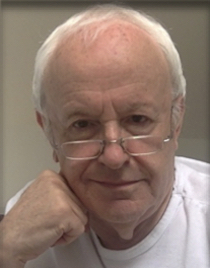
\includegraphics[width=2.19in]{assets/RPF-thumbnail} \caption{This image should really be one that nicely summarises your topic. Not Roger.}\label{fig:rpmain}
\end{figure}

\section*{Keynote Lecture}\label{keynote-lecture}
\addcontentsline{toc}{section}{Keynote Lecture}

\subsection*{Jijie Chai - Structural Study of Plant Receptor
Kinases}\label{jijie-chai---structural-study-of-plant-receptor-kinases}
\addcontentsline{toc}{subsection}{Jijie Chai - Structural Study of Plant
Receptor Kinases}

\textbf{Max Planck Institute for Breeding Research, University of
Cologne}

Plant receptor kinases (RKs) are a large family of single transmembrane
proteins that play important roles in diverse biological processes
including development, growth and immunity. RKs are characterized with
diversified extracellular domains (ECDs) and conserved intracellular
kinase domains. Recognition of their cognate ligands by ECDs of RKs
initiates activation of RKs. The molecular mechanisms underlying this
process remained poorly defined. We recently solved the crystal
structures of the ECDs derived from several RKs in complex with their
respective ligands. These structures define the molecular mechanisms by
which these RKs recognize their specific ligands. More importantly, a
general mechanism underlying ligand-induced activation of RKs can be
formulated. In the current talk, I will briefly review what we have done
on structural study of RKs and present two examples of how RK activation
and ligand recognition mechanisms were used for the matching of
receptor-ligand pairs.

\subsection*{About Jijie Chai}\label{about-jijie-chai}
\addcontentsline{toc}{subsection}{About Jijie Chai}

\begin{quote}
Jijie Chai was born on April 16, 1966 in Liaoning province, China. He
received his bachelor's degree in chemical engineering from Dalian Light
Industry College, master's degree in applied chemistry from the Research
Institute of Petroleum Processing (Beijing) and Ph.D.~in analytical
chemistry from the Institute of Materia Medica, Chinese Academy of
Medical Sciences and Peking Union Medical College.

From 1999 to 2004, he worked as postdoctoral fellow at Princeton
University, where he started his research in structural biology.

In July 2004, he joined the National Institute of Biological Sciences as
an independent investigator, where he established his own research
programs, structural study of plant receptor kinases and NOD-like
receptors. After working there for six and half years, he moved to
Tsinghua University and continued his research as a full professor.

Early last year, he was awarded with the Alexander von Humboldt
Professorship, and he moved to Cologne late March of 2017. Jijie has
published a number of papers on RLKs and NLRs, advancing our
understanding the mechanisms of RLK activation and NLR inhibition and
activation.

Jijie is happily married and the father of a daughter. He is currently
living in Cologne.
\end{quote}

\section*{Practical Session - Model pathosystems and effector triggered
immunity
readouts}\label{practical-session---model-pathosystems-and-effector-triggered-immunity-readouts}
\addcontentsline{toc}{section}{Practical Session - Model pathosystems
and effector triggered immunity readouts}

\textbf{Led by Zane Duxbury}

\subsection*{Aims and Objectives}\label{aims-and-objectives}
\addcontentsline{toc}{subsection}{Aims and Objectives}

\begin{enumerate}
\def\labelenumi{\arabic{enumi}.}
\tightlist
\item
  Become familiar with using model organisms to probe the plant immune
  system
\item
  Understand and recognise the lifecycle and symptoms of some common
  diseases
\item
  Understand transient expression systems for determining relationship
  between \textbf{R} and \textbf{avirulence} genes
\end{enumerate}

The plant immune system contains both cell surface and intracellular
receptors. Cell surface receptors often confer broad spectrum
recognition to conserved pathogen-associated molecular patterns (PAMPs),
and upon recognition the plant mounts an immune response termed
PAMP-triggered immunity (PTI). Pathogens co-evolve with their hosts and
can overcome PTI through the evolution of proteins they secrete into
plants, termed effectors, which suppress components of the PTI
machinery. Plant intracellular receptors can detect effectors by binding
them directly or by indirectly recognising their activity; this
recognition triggers a strong immune response (effector-trigger
immunity; ETI) that shares molecular components with PTI but is often
stronger and is characterized by a cell-death response termed the
hypersensitive response (HR). A recognised effector leads to loss of
virulence in resistant plants with the cognate intracellular receptor,
and is hence termed an avirulence factor (Avr) in this case. The
intracellular receptors are encoded by Resistance (R) genes that have
been strongly selected for by plant breeders for the strain-specific
resistance conferred to pathogens that have broken other resistance
mechanisms. This co-evolution of pathogen virulence versus plant
immunity is encompassed by the zig-zag model of plant immunity (Figure
\ref{fig:zigzag} )










\begin{figure}
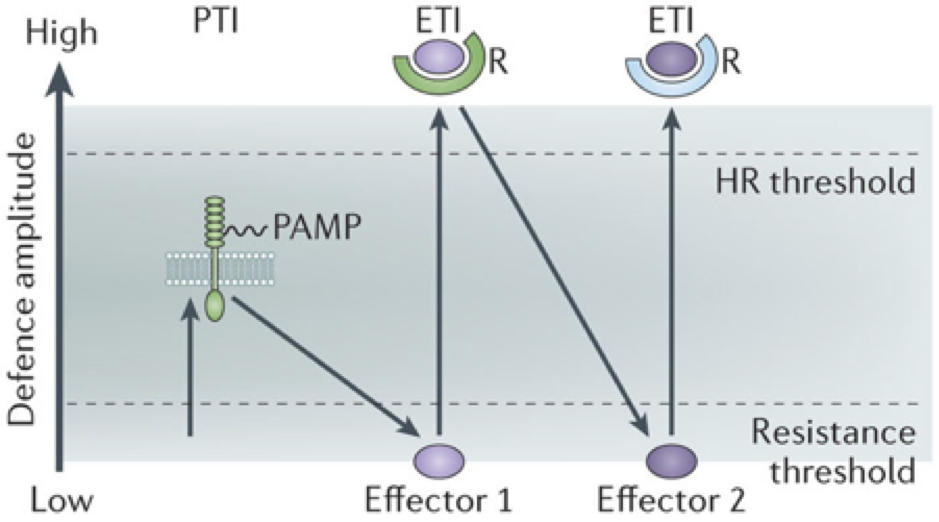
\includegraphics[width=9.78in]{assets/jones_fig1_prac} \caption{The zig-zag model of plant immunity \citep{Jones:2006ih}.
The ultimate amplitude of defence is the combined sum of resistance
output (ETI+PTI) and the difference of the effect of pathogen effectors
(-ETS; effector triggered susceptibility). This diagram captures the
observation that many PTI and ETI outputs are similar, but HR is
associated specifically with successful ETI, and that virulent pathogens
with specific effectors are able to suppress immunity to compromise
immunity. Image is from \citet{Pumplin:2013ix}.}\label{fig:zigzag}
\end{figure}

The aim of this practical session will be to familiarise you with the
use of model organisms to probe the plant immune system. The practical
will include a general introduction to the oomycete pathogens of
Arabidopsis: \emph{Albugo spp} and \emph{Hyaloperonospora arabidopsidis}
(white rust and downy mildew respectively), the bacterial species
\emph{Pseudomonas syringae} and \emph{P. fluorescens}, and the
pathosystem of potato and the oomycete \emph{Phytophthora infestans}
(late blight) (Figure \ref{fig:leaves}).

We will familiarise you with the life cycle, pathogenesis and symptoms
of these pathogens. We will use various techniques to assess the growth
of pathogens on their hosts and to assess immune responses mounted
against these pathogens. For example, we will use light microscopy of
trypan-blue stained Arabidopsis infected with downy mildew to
qualitatively assess the success of infection and resistance of
different genotypes of the pathogen and plant. We will introduce
transient expression systems such as bombardment and \emph{Agrobacterium
tumefaciens}-mediated \emph{Nicotiana tabacum} transformation
(agroinfiltration) to determine the relationship between R- and
avirulence-genes responsible for compatible (resulting in disease) or
incompatible (resulting in healthy plants) interactions.











\begin{figure}
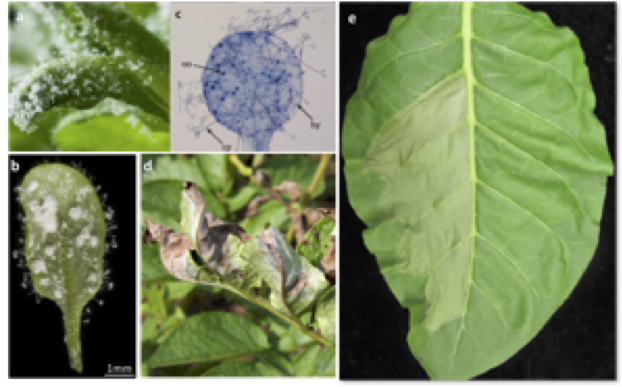
\includegraphics[width=6.48in]{assets/jones_fig2_prac} \caption{Macroscopic characteristics of plant-pathogen
interactions. a, b) Sporulating Hyaloperonospora arabidopsidis (seen on
the edges of the leaf in b) growing on \emph{Arabidopsis thaliana}
leaves. Albugo is also growing on the abaxial surface of the leaf in b.
c) Trypan blue staining of a \emph{H. arabidopsidis-infected} leaf of
Arabidopsis. d) Foliar symptoms of \emph{Phytophthora infestans}
infection of potato. e) Hypersensitive cell death in tobacco leaf
resulting from \emph{Agrobacterium tumefaciens}-mediated transformation
with cognate R gene and Avr gene.}\label{fig:leaves}
\end{figure}

\chapter*{Genomic Resources and Bioinformatics for Plant Microbe
Interactions.}\label{genomic-resources-and-bioinformatics-for-plant-microbe-interactions.}
\addcontentsline{toc}{chapter}{Genomic Resources and Bioinformatics for
Plant Microbe Interactions.}

\textbf{Led by Dan MacLean}

The increase in the generation and analysis of sequence data in the last
ten years has had a profound effect on plant and microbe interaction
research. The genomes of the wide range of host and pathogen's of
interest are now open to study in a way that is within reach of most
scientists - not just large genome sequencing institutes - and many
laboratories are now undertaking genomics as a routine approach.

The deluge of data created by new sequencing approaches has been
collected into a wide range of general and domain specific databases,
each of which contain different information accessed in different ways.
Knowing which are the most useful databases in a given context is
therefore a tricky question and in this session we will take a tour of
the most widely-used including \href{http://ensembl.org}{Ensembl},
\href{http://phytopathdb.org}{PhytoPath},
\href{http://solgenomics.net}{SolGenomics},
\href{http://arabidopsis.org}{TAIR} and
\href{http://araport.org}{AraPort}.

Sequence data are used in a wide range of applications and the source
molecule will be selected in an application specific way. Genomic DNA is
used for assembly of draft genomes, RNA is used for gene expression
analysis, genome annotation and exome construction. Both DNA and RNA get
used to identify genetic polymorphisms. Mixed populations of nucleic
acids from environmental (e.g soil or pathogen/host interaction sites)
are used to study species compositions. A wide range of bioinformatics
tools have been developed and are in common use for these approaches, so
in this topic we will study briefly the tools and their core algorithms
and competencies with the aim of helping you to decide on the right
tools for any particular analysis that you may wish to do outside of the
course. A useful guide is available in \citet{MacLean:2009hm}. In
particular we will look at algorithms and tools for \emph{de novo}
assembly of sequence including SOAPdenovo \citep{Luo:2012fn} and
\href{http://wgs-assembler.sourceforge.net/wiki/index.php?title=Main_Page}{Celera
Assembler}. We will study tools for RNASeq expression and annotation
analyses including Tophat \citep{Trapnell:2009dp} and Bowtie
\citep{Langmead:2012jh} and DESeq \citep{Anders:2010fu} and edgeR
\citep{Robinson:2010cw}.







\begin{figure}
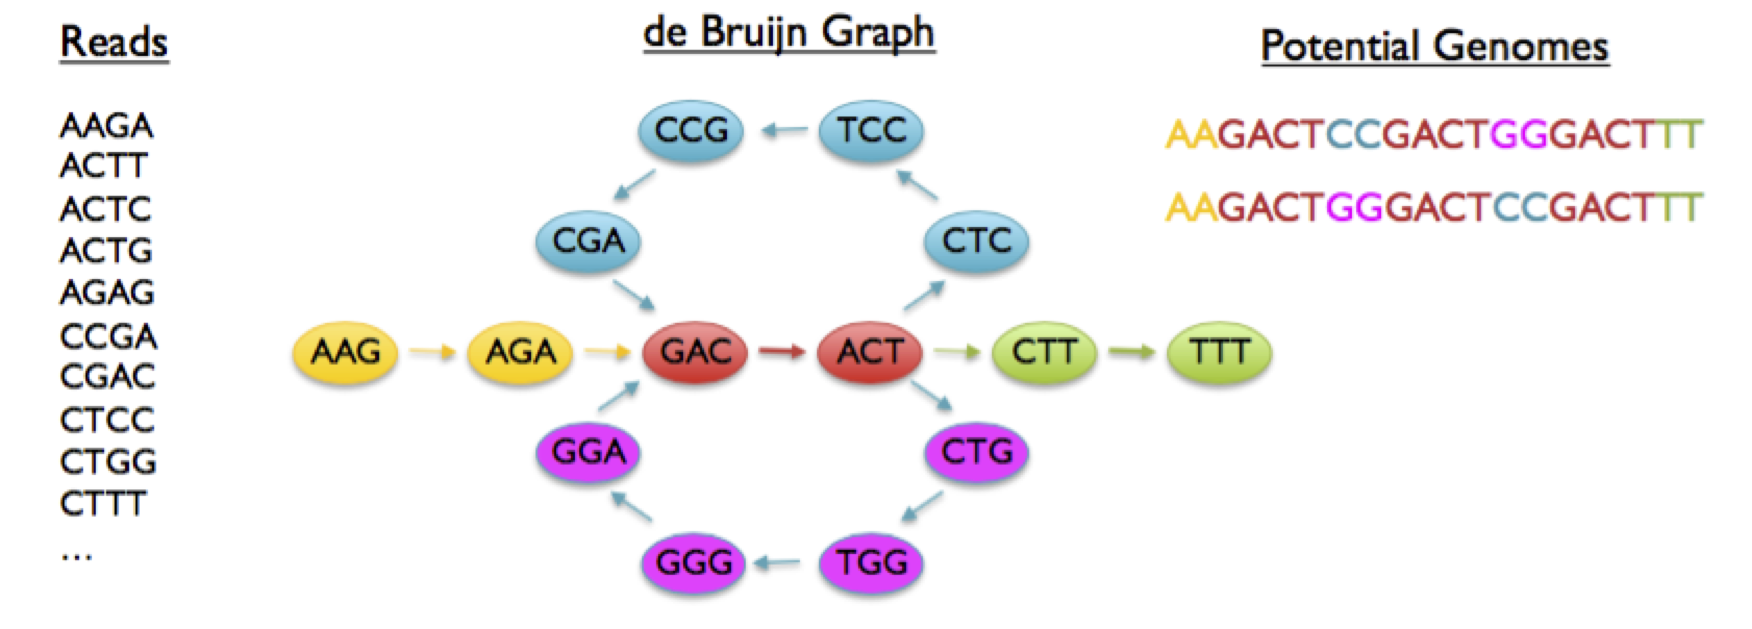
\includegraphics[width=7.01in]{assets/algo} \caption{Graphical summary of a \emph{de novo} assembly algorithm.
Sequence reads are broken down into constituent \emph{k}-mers and a
network of overlapping \emph{k}-mers is produced. The paths in the graph
are traversed and the \emph{k}-mers collected into a growing string
representing a long sequence in the original data and therefore genome.}\label{fig:mainbio}
\end{figure}

\section*{Keynote Lecture}\label{keynote-lecture-1}
\addcontentsline{toc}{section}{Keynote Lecture}

\subsection*{Diane Saunders - Field
Pathogenomics}\label{diane-saunders---field-pathogenomics}
\addcontentsline{toc}{subsection}{Diane Saunders - Field Pathogenomics}

\textbf{John Innes Centre, Norwich, UK}

\subsection*{About Diane Saunders}\label{about-diane-saunders}
\addcontentsline{toc}{subsection}{About Diane Saunders}

\begin{quote}
bio bio bio
\end{quote}

\section*{Practical Session - From Sequence Data to Candidate
Protein}\label{practical-session---from-sequence-data-to-candidate-protein}
\addcontentsline{toc}{section}{Practical Session - From Sequence Data to
Candidate Protein}

\textbf{Led by Dan MacLean}

\subsection*{Aims and Objectives}\label{aims-and-objectives-1}
\addcontentsline{toc}{subsection}{Aims and Objectives}

\begin{enumerate}
\def\labelenumi{\arabic{enumi}.}
\tightlist
\item
  Understand Strengths and Weaknesses of High Throughput Sequence Data
\item
  Know how to call SNPs from HTS data on
\item
  Categorise SNPs according to an expected genetic background
\end{enumerate}

Genomics has come a long way. We can now sequence genomes quickly and to
a reasonable degree of accuracy. We can create in a high-throughput
manner an inventory of sub-regions in a genome that we think are genes.
We know the functions (or some of the functions) of lots of genes and we
can infer functions of newly discovered genes by comparison of sequence
or structure, basically by seeing whether our new thing looks like
something else.

These methods are actually only PREDICTIONS of function. Looking a bit
like something else is only a clue to what something does. It frequently
fails us.

In this practical we will look at the powerful technique of mutational
genomics. This is possibly the coolest thing ever as it involves
mutating a living organism so that it is different from other things and
then sequencing the genome to pinpoint the exact changes that cause the
difference. We don't have the scope or chemicals to do the mutation bit,
so we'll pick up with the genomics and use Galaxy and Galaxy tools to
carry out the analysis that takes us from sequence data to actual
candidate mutations in the genome sequence.

With mutational genomics we deal initially with the effect of the gene
on the whole organism. By performing mutagenesis on our favourite
organism then carrying out a genetic screen \citep{Page:2002ji} that
selects individuals that have changed in the phenotype we are interested
in, we have our first foothold on function. We can study those
individuals and apply the principles of genetics, use modern
high-throughput sequencing and bioinformatics tools to identify the gene
causing that phenotype change (or at least ones involved in the process
we have messed up).

We will use tools in the Galaxy \citep{Goecks:2010ea} framework
including FastQC for quality control of sequence data (Figure
\ref{fig:fqc}) \citep{FastQC}, BWA for read mapping and alignment
\citep{Li:2009fi} and CandiSNP \citep{Etherington:2014ba} to identify
candidate mutations (Figure \ref{fig:candisnp}) .

\begin{figure}
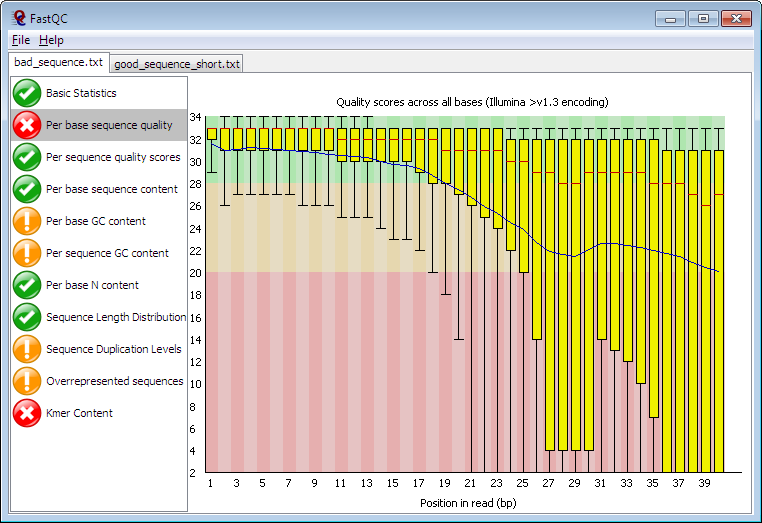
\includegraphics[width=5.08in]{assets/fastqc} \caption{FastQC Quality Control of sequence reads}\label{fig:fqc}
\end{figure}

\begin{figure}
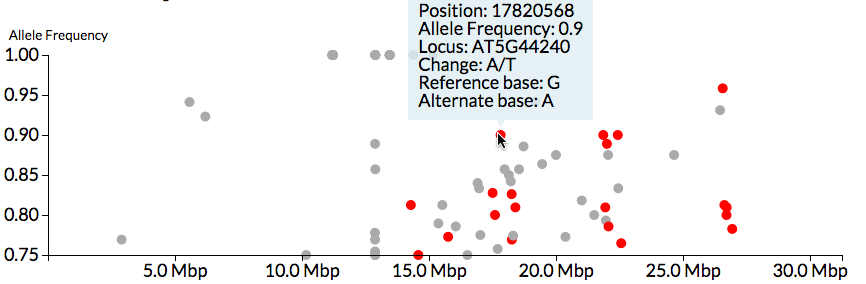
\includegraphics[width=5.77in]{assets/candisnp} \caption{CandiSNP visualisation of SNPs}\label{fig:candisnp}
\end{figure}

\chapter*{Effectors and Immunity}\label{effectors-and-immunity}
\addcontentsline{toc}{chapter}{Effectors and Immunity}

\textbf{Led by Sophien Kamoun}

Lorem ipsum dolor sit amet, consectetur adipiscing elit. In iaculis
sagittis metus quis malesuada. Vestibulum laoreet vel tortor at tempor.
Mauris blandit volutpat risus, et placerat odio varius eget. Cras vitae
diam sollicitudin justo vehicula ultrices. Curabitur consequat ornare
odio ac hendrerit. Mauris bibendum diam nec gravida molestie. Nullam
interdum, nulla eget sollicitudin elementum, ante lorem auctor odio, sit
amet varius diam magna et lectus. Sed vehicula velit velit, convallis
mollis erat laoreet nec. Cras semper blandit felis vel iaculis. Sed in
mollis nulla. Nulla sed egestas odio, nec finibus lectus. In vel
porttitor lacus, nec tincidunt neque. Suspendisse at magna non neque
congue fermentum at ut augue. Vivamus suscipit finibus tortor, ut
accumsan dui pretium nec. Integer luctus eros non convallis ornare.

Pellentesque dapibus arcu rutrum neque tempor, ac consequat nisi
consectetur. Nunc eu tortor sed lorem vehicula finibus. Sed sed lacus at
erat fringilla auctor. Aenean malesuada mi est, sit amet molestie ante
malesuada in. Aenean elit risus, imperdiet quis pretium ac, imperdiet a
turpis. Praesent cursus, orci a viverra tincidunt, augue tortor volutpat
erat, a elementum nisi ante vel nisl. Vestibulum purus nisl, imperdiet
egestas ultricies nec, tempor vitae ligula. Integer dapibus magna vitae
orci pharetra rhoncus. Vestibulum in mauris feugiat, pulvinar massa ac,
convallis lacus. In hac habitasse platea dictumst.

Aenean sed leo sit amet dolor congue semper. Curabitur non malesuada
erat. Phasellus scelerisque rutrum tristique. Duis posuere quam tellus,
eu posuere lorem convallis facilisis. Duis euismod tincidunt neque, eu
pellentesque nisi mollis sed. Suspendisse eu nunc rutrum massa iaculis
rhoncus rutrum nec velit. Nulla et erat quis urna malesuada auctor.
Vestibulum sit amet diam maximus, luctus nulla mollis, vestibulum nisi.

\begin{figure}
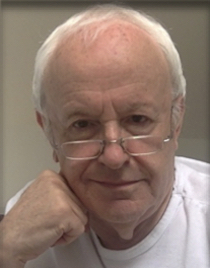
\includegraphics[width=2.19in]{assets/RPF-thumbnail} \caption{This image should really be one that nicely summarises your topic. Not Roger.}\label{fig:maineff}
\end{figure}

\section*{Keynote Lecture}\label{keynote-lecture-2}
\addcontentsline{toc}{section}{Keynote Lecture}

\subsection*{Keynote Speaker Name - Keynote Speaker
Title}\label{keynote-speaker-name---keynote-speaker-title}
\addcontentsline{toc}{subsection}{Keynote Speaker Name - Keynote Speaker
Title}

\textbf{Keynote Speaker Affiliation}

\subsection*{About Keynote Speaker}\label{about-keynote-speaker}
\addcontentsline{toc}{subsection}{About Keynote Speaker}

\begin{quote}
bio bio bio
\end{quote}

\section*{Practical Session - Practical Session
Title}\label{practical-session---practical-session-title}
\addcontentsline{toc}{section}{Practical Session - Practical Session
Title}

\textbf{Led by Practical Session Lead}

\subsection*{Aims and Objectives}\label{aims-and-objectives-2}
\addcontentsline{toc}{subsection}{Aims and Objectives}

\begin{enumerate}
\def\labelenumi{\arabic{enumi}.}
\tightlist
\item
  Teach
\item
  Learn
\item
  Profit
\end{enumerate}

Lorem ipsum dolor sit amet, consectetur adipiscing elit. In iaculis
sagittis metus quis malesuada. Vestibulum laoreet vel tortor at tempor.
Mauris blandit volutpat risus, et placerat odio varius eget. Cras vitae
diam sollicitudin justo vehicula ultrices. Curabitur consequat ornare
odio ac hendrerit. Mauris bibendum diam nec gravida molestie. Nullam
interdum, nulla eget sollicitudin elementum, ante lorem auctor odio, sit
amet varius diam magna et lectus. Sed vehicula velit velit, convallis
mollis erat laoreet nec. Cras semper blandit felis vel iaculis. Sed in
mollis nulla. Nulla sed egestas odio, nec finibus lectus. In vel
porttitor lacus, nec tincidunt neque. Suspendisse at magna non neque
congue fermentum at ut augue. Vivamus suscipit finibus tortor, ut
accumsan dui pretium nec. Integer luctus eros non convallis ornare.

Pellentesque dapibus arcu rutrum neque tempor, ac consequat nisi
consectetur. Nunc eu tortor sed lorem vehicula finibus. Sed sed lacus at
erat fringilla auctor. Aenean malesuada mi est, sit amet molestie ante
malesuada in. Aenean elit risus, imperdiet quis pretium ac, imperdiet a
turpis. Praesent cursus, orci a viverra tincidunt, augue tortor volutpat
erat, a elementum nisi ante vel nisl. Vestibulum purus nisl, imperdiet
egestas ultricies nec, tempor vitae ligula. Integer dapibus magna vitae
orci pharetra rhoncus. Vestibulum in mauris feugiat, pulvinar massa ac,
convallis lacus. In hac habitasse platea dictumst.

\chapter*{Surface Immunity}\label{surface-immunity}
\addcontentsline{toc}{chapter}{Surface Immunity}

\textbf{Led by Cyril Zipfel}

The first layer of plant innate immunity depends on the recognition of
microbes via the perception of pathogen-associated molecular patterns
(PAMPs) or damage-associated molecular patterns (DAMPs) by plasma
membrane-localized pattern recognition receptors (PRRs). Plant PRRs are
ligand-binding receptor kinases or receptor-like proteins that exist in
multi-protein complexes to transduce intracellular immune signaling by
triggering downstream phosphorylation cascades \citep{Couto:2016kq}. The
Arabidopsis leucine-rich repeat receptor kinases (LRR-RKs) FLS2 and EFR
are well-studied PRRs that bind the bacterial PAMPs flagellin and EF-Tu
(or their immunogenic epitopes flg22 and elf18), respectively. In both
cases, ligand-binding triggers rapid hetero-oligomerization with SERK
co-receptors. Of these, BAK1/SERK3 and its closest paralog BKK1/SERK4
are the major regulators of FLS2- and EFR-dependent signaling.
Intriguingly, BAK1 and other SERKs are also involved in various
non-immune signaling pathways \citep{Ma:2016eu}. An allele of BAK1
specifically affected in PTI, bak1-5, enabled the uncoupling of BAK1's
functions in PTI, brassinosteroid (BR) signaling and cell death control
\citep{Schwessinger:2011ku}, allowing a detailed characterization of
BAK1 in immune signaling without the influence of the morphological
defects observed for other BAK1

The plasma membrane-associated receptor-like cytoplasmic kinase (RLCK)
BIK1 is an immediate convergent substrate of several different PRRs as
well as BAK1 \citep{Couto:2016kq}. In response to PAMP perception, BIK1
is phosphorylated and released from the receptor complex and
subsequently phosphorylates the NADPH oxidase RBOHD, which is required
to produce reactive oxygen species (ROS), one of the first hallmark
responses triggered after PAMP perception
\citep{Kadota:2014bi, Li:2014dx}. Another early PTI response is the
influx of apoplastic Ca2+2+via yet unknown channels, a response that is
also BIK1-dependent \citep{Li:2014dx, Ranf:2014fg, Seybold:2014wt}.
Subsequently, PAMP perception results in the activation of a MAP kinase
cascade and calcium-dependent protein kinases, which ultimately results
in the transcriptional reprogramming of the cell - mostly via WRKY
transcription factors - and ultimately to the restriction of pathogen
growth \citep{Couto:2016kq}. Later responses associated with FLS2 and
EFR activation include increased ethylene biosynthesis, callose
deposition, and inhibition of seedling growth \citep{Boller:2009hu}.

\begin{figure}
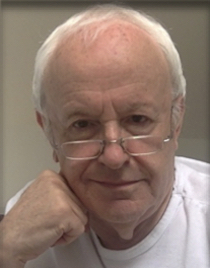
\includegraphics[width=2.19in]{assets/RPF-thumbnail} \caption{This image should really be one that nicely summarises your topic. Not Roger.}\label{fig:mainsi}
\end{figure}

\section*{Keynote Lecture}\label{keynote-lecture-3}
\addcontentsline{toc}{section}{Keynote Lecture}

\subsection*{Stefanie Ranf - Signalling in Plant Innate
Immunity}\label{stefanie-ranf---signalling-in-plant-innate-immunity}
\addcontentsline{toc}{subsection}{Stefanie Ranf - Signalling in Plant
Innate Immunity}

\textbf{Technische Universitat Munchen}

\subsection*{About Stefanie Ranf}\label{about-stefanie-ranf}
\addcontentsline{toc}{subsection}{About Stefanie Ranf}

\begin{quote}
bio bio bio
\end{quote}

\section*{Practical Session - Analysing Surface
Immunity}\label{practical-session---analysing-surface-immunity}
\addcontentsline{toc}{section}{Practical Session - Analysing Surface
Immunity}

\textbf{Led by Martin Stegmann}

\subsection*{Aims and Objectives}\label{aims-and-objectives-3}
\addcontentsline{toc}{subsection}{Aims and Objectives}

\begin{enumerate}
\def\labelenumi{\arabic{enumi}.}
\tightlist
\item
  Understanding of and hands on experience in classical methods to
  analyse PTI responses in the model organism \emph{Arabidopsis
  thaliana}
\item
  Testing the importance of critical PTI regulators, mainly by analysing
  the impact of PRRs and PRR-associated RLKs on the activation of PTI
  signalling
\item
  Understanding the contribution of PTI on plant immunity against
  adapted bacterial pathogens
\end{enumerate}

The practical session ``Analysing Surface Immunity'' will consist of a
pedagogical lecture on the biochemical and molecular biological
techniques used to investigate the molecular basis of PTI signaling, and
to identify novel PAMPs or PRRs. We will demonstrate some of the
classical methods used to analyze downstream PTI responses, such as ROS
production, MAPK activation, seedling growth inhibition and surface
immunity upon spray infection with bacterial pathogens.

For measuring the PAMP-triggered ROS burst, we will make use of a
luminescence based assay, which enables the detection of apoplastic ROS
in a light-based reaction that can be monitored live with a
charge-coupled device camera. This is a fast and easy quantitative assay
that can be used, in many cases, to study early PTI signalling in a
given mutant compared to a wild type control.

In addition, we will assay for the induction of a MAPK cascade,
specifically for the PAMP-induced phosphorylation of the four
Arabidopsis MAPKs MPK3, MPK4, MPK6 and MPK11. Their activation can be
detected a few minutes after PAMP treatment by Western blot analysis
using a well-established commercial antibody that was raised to detect
phosphorylated MAPKs in mammalian systems.

Prolonged exposure to PAMPs results in a growth arrest of seedlings,
which can be used as a quantitative measure for the capability of a
given genotype to respond to different stimuli. We will take a look at
different Arabidopsis lines exposed to PAMPs for several days and assess
the resulting growth differences compared to mock grown seedlings.
Finally, PAMP-triggered immunity contributes to the basal resistance of
plants against adapted pathogens. In the frame of the practical session
we will assess the differences in susceptibility of known PTI pathway
mutants to demonstrate the importance of PTI for plant resistance.

\chapter*{Cellular Defence}\label{cellular-defence}
\addcontentsline{toc}{chapter}{Cellular Defence}

\textbf{Led by Silke Robatzek}

Lorem ipsum dolor sit amet, consectetur adipiscing elit. In iaculis
sagittis metus quis malesuada. Vestibulum laoreet vel tortor at tempor.
Mauris blandit volutpat risus, et placerat odio varius eget. Cras vitae
diam sollicitudin justo vehicula ultrices. Curabitur consequat ornare
odio ac hendrerit. Mauris bibendum diam nec gravida molestie. Nullam
interdum, nulla eget sollicitudin elementum, ante lorem auctor odio, sit
amet varius diam magna et lectus. Sed vehicula velit velit, convallis
mollis erat laoreet nec. Cras semper blandit felis vel iaculis. Sed in
mollis nulla. Nulla sed egestas odio, nec finibus lectus. In vel
porttitor lacus, nec tincidunt neque. Suspendisse at magna non neque
congue fermentum at ut augue. Vivamus suscipit finibus tortor, ut
accumsan dui pretium nec. Integer luctus eros non convallis ornare.

\begin{figure}
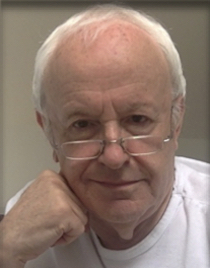
\includegraphics[width=2.19in]{assets/RPF-thumbnail} \caption{This image should really be one that nicely summarises your topic. Not Roger.}\label{fig:maincd}
\end{figure}

\section*{Keynote Lecture}\label{keynote-lecture-4}
\addcontentsline{toc}{section}{Keynote Lecture}

\subsection*{Paul Birch - Keynote Speaker
Title}\label{paul-birch---keynote-speaker-title}
\addcontentsline{toc}{subsection}{Paul Birch - Keynote Speaker Title}

\textbf{James Hutton Institute, Dundee, UK}

\subsection*{About Paul Birch}\label{about-paul-birch}
\addcontentsline{toc}{subsection}{About Paul Birch}

\begin{quote}
bio bio bio
\end{quote}

\section*{Practical Session - Live Cell Imaging and Investigation of
Subcellular Membrane
Trafficking}\label{practical-session---live-cell-imaging-and-investigation-of-subcellular-membrane-trafficking}
\addcontentsline{toc}{section}{Practical Session - Live Cell Imaging and
Investigation of Subcellular Membrane Trafficking}

\textbf{Led by} \href{gildas.bourdais@sainsbury-laboratory.ac.uk}{Gildas
Bourdais}, \href{michaela.kopischke@sainsbury-laboratory.ac.uk}{Michaela
Kopischke},
\href{agnieszka.siwoszek@sainsbury-laboratory.ac.uk}{Agnieszka
Siwoszek}, \href{jelle.postma@sainsbury-laboratory.ac.uk}{Jelle Postma},
\href{katarzyna.rybak@sainsbury-laboratory.ac.uk}{Katarzyna Rybak},
\href{janina.tamborski@sainsbury-laboratory.ac.uk}{Janina Tamborski}

\subsection*{Aims and Objectives}\label{aims-and-objectives-4}
\addcontentsline{toc}{subsection}{Aims and Objectives}

\begin{enumerate}
\def\labelenumi{\arabic{enumi}.}
\tightlist
\item
  Perform advanced fluorescence imaging using confocal laser scanning
  and spinning disc microscopy
\item
  Generate images suitable for qualitative and quantitative analyses
\item
  Provide a tool-box to understand and study the plant's endomembrane
  trafficking machinery
\end{enumerate}

Plants mount multi-layered immune responses that comprise passive and
active defences. Plasma membrane (PM) localised pattern recognition
receptors (PRRs) enable plants to perceive Pathogen-Associated Molecular
Patterns (PAMPs) displayed by potential microbial invaders to activate
defence responses. The PRR FLAGELLIN SENSING2 (FLS2) confers immunity
against bacterial infection through perception of a 22 amino acid
epitope of flagellin (flg22).

In recent years the importance of PRR subcellular trafficking to plant
immunity has become apparent. PRRs are secreted through the
endoplasmatic reticulum (ER) and the Golgi apparatus to the plasma
membrane, where they recognize their cognate ligands. At the plasma
membrane, PRRs can be recycled or internalized via endocytic pathways.
The endocytic pathway in plants comprises early and late endocytic
compartments.

FLS2 constitutes a well-known example to study endocytic trafficking.
From the PM FLS2 is internalized in a clathrin-dependent manner and
targeted towards distinct subcellular fates in dependence of its
activation status. At the stage of the trans-golgi-network (TGN)/ early
endosome (EE) non-activated FLS2 is recycled back to the plasma
membrane. Activated (flg22-bound) FLS2 is sorted to the late endosomal
pathway and internalized into intra-luminal vesicles of multi-vesicular
bodies (MVBs) destined for vacuolar degradation, which is regulated by
the endosomal sorting complexes required for transport (ESCRT) sorting
machinery (See Figure \ref{fig:srfig} a).

Mutants lacking clathrin- or ESCRT- components are more susceptible to
bacterial infection, indicating the importance of endomembrane
trafficking regulators for the establishment of efficient defence
responses.

Small Rab GTPases and Syntaxins act at multiple stages of vesicle
trafficking, including cargo selection, vesicle formation, vesicle
movement, tethering and membrane fusion. Distinct members of these
families are associated with specific membrane compartments. Therefore
these proteins, such as the Rab5 GTPases ARA6 and ARA7 or the syntaxin
SYP61 which are localised at the MVB/LE-, EE/LE and TGN, respectively),
can be used as marker proteins to identify specific membrane
compartments.

In the practical sessions we will investigate the (co-)localisation of
FLS2-GFP and various endosomal marker proteins following flg22 treatment
using live-cell imaging approaches (See Figure \ref{fig:srfig} b).
Chemical inhibitors and genetic interference with the endomembrane
trafficking machinery will help us to dissect and understand the route
of activated FLS2 in a temporal and spatial resolution.












\begin{figure}
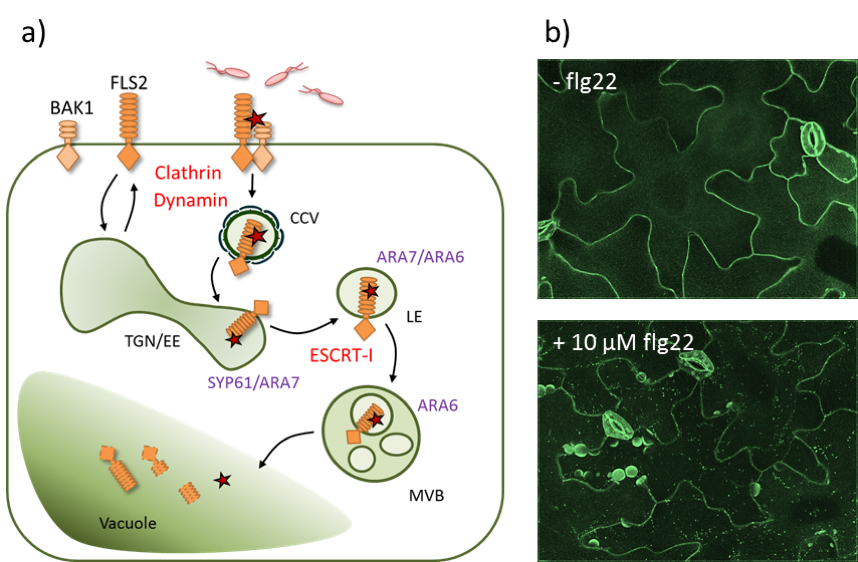
\includegraphics[width=5.72in]{assets/sr_fig1_prac} \caption{FLS2 endocytsosis. \textbf{a)} The PRR FLS2 and its
co-receptor BAK1 localise at the plasma membrane. Upon flg22 perception,
a receptor complex is formed and the activated receptor is internalised
into clathrin-coated vesicles (CCV) and sorted into intraluminal
vesicles of multi-vesicular bodies (MVBs) via the trans-Golgi-network
(TGN)/early endosomes (EE) and the late endosomes (LE). Components
required for FLS2 internalisation and sorting are indicated in red,
endosomal marker proteins are indicated in lilac. \textbf{b)} Confocal
micrographs (spinning disc microscopy) of FLS2-GFP before and after
elicitation with flg22.}\label{fig:srfig}
\end{figure}

\chapter*{Wheat Genomics}\label{wheat-genomics}
\addcontentsline{toc}{chapter}{Wheat Genomics}

\textbf{Led by Ksenia Krasileva}

\emph{Adopting new wheat genomic tools to dissect plant innate immunity}

Lorem ipsum dolor sit amet, consectetur adipiscing elit. In iaculis
sagittis metus quis malesuada. Vestibulum laoreet vel tortor at tempor.
Mauris blandit volutpat risus, et placerat odio varius eget. Cras vitae
diam sollicitudin justo vehicula ultrices. Curabitur consequat ornare
odio ac hendrerit. Mauris bibendum diam nec gravida molestie. Nullam
interdum, nulla eget sollicitudin elementum, ante lorem auctor odio, sit
amet varius diam magna et lectus. Sed vehicula velit velit, convallis
mollis erat laoreet nec. Cras semper blandit felis vel iaculis. Sed in
mollis nulla. Nulla sed egestas odio, nec finibus lectus. In vel
porttitor lacus, nec tincidunt neque. Suspendisse at magna non neque
congue fermentum at ut augue. Vivamus suscipit finibus tortor, ut
accumsan dui pretium nec. Integer luctus eros non convallis ornare.

Pellentesque dapibus arcu rutrum neque tempor, ac consequat nisi
consectetur. Nunc eu tortor sed lorem vehicula finibus. Sed sed lacus at
erat fringilla auctor. Aenean malesuada mi est, sit amet molestie ante
malesuada in. Aenean elit risus, imperdiet quis pretium ac, imperdiet a
turpis. Praesent cursus, orci a viverra tincidunt, augue tortor volutpat
erat, a elementum nisi ante vel nisl. Vestibulum purus nisl, imperdiet
egestas ultricies nec, tempor vitae ligula. Integer dapibus magna vitae
orci pharetra rhoncus. Vestibulum in mauris feugiat, pulvinar massa ac,
convallis lacus. In hac habitasse platea dictumst.

Aenean sed leo sit amet dolor congue semper. Curabitur non malesuada
erat. Phasellus scelerisque rutrum tristique. Duis posuere quam tellus,
eu posuere lorem convallis facilisis. Duis euismod tincidunt neque, eu
pellentesque nisi mollis sed. Suspendisse eu nunc rutrum massa iaculis
rhoncus rutrum nec velit. Nulla et erat quis urna malesuada auctor.
Vestibulum sit amet diam maximus, luctus nulla mollis, vestibulum nisi.

\begin{figure}
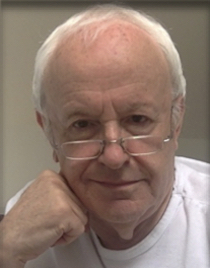
\includegraphics[width=2.19in]{assets/RPF-thumbnail} \caption{This image should really be one that nicely summarises your topic. Not Roger.}\label{fig:mainwg}
\end{figure}

\section*{Keynote Lecture}\label{keynote-lecture-5}
\addcontentsline{toc}{section}{Keynote Lecture}

\subsection*{Keynote Speaker Name - Keynote Speaker
Title}\label{keynote-speaker-name---keynote-speaker-title-1}
\addcontentsline{toc}{subsection}{Keynote Speaker Name - Keynote Speaker
Title}

\textbf{Keynote Speaker Affiliation}

\subsection*{About Keynote Speaker}\label{about-keynote-speaker-1}
\addcontentsline{toc}{subsection}{About Keynote Speaker}

\begin{quote}
bio bio bio
\end{quote}

\section*{Practical Session - Practical Session
Title}\label{practical-session---practical-session-title-1}
\addcontentsline{toc}{section}{Practical Session - Practical Session
Title}

\textbf{Led by Practical Session Lead}

\subsection*{Aims and Objectives}\label{aims-and-objectives-5}
\addcontentsline{toc}{subsection}{Aims and Objectives}

\begin{enumerate}
\def\labelenumi{\arabic{enumi}.}
\tightlist
\item
  Teach
\item
  Learn
\item
  Profit
\end{enumerate}

Lorem ipsum dolor sit amet, consectetur adipiscing elit. In iaculis
sagittis metus quis malesuada. Vestibulum laoreet vel tortor at tempor.
Mauris blandit volutpat risus, et placerat odio varius eget. Cras vitae
diam sollicitudin justo vehicula ultrices. Curabitur consequat ornare
odio ac hendrerit. Mauris bibendum diam nec gravida molestie. Nullam
interdum, nulla eget sollicitudin elementum, ante lorem auctor odio, sit
amet varius diam magna et lectus. Sed vehicula velit velit, convallis
mollis erat laoreet nec. Cras semper blandit felis vel iaculis. Sed in
mollis nulla. Nulla sed egestas odio, nec finibus lectus. In vel
porttitor lacus, nec tincidunt neque. Suspendisse at magna non neque
congue fermentum at ut augue. Vivamus suscipit finibus tortor, ut
accumsan dui pretium nec. Integer luctus eros non convallis ornare.

Pellentesque dapibus arcu rutrum neque tempor, ac consequat nisi
consectetur. Nunc eu tortor sed lorem vehicula finibus. Sed sed lacus at
erat fringilla auctor. Aenean malesuada mi est, sit amet molestie ante
malesuada in. Aenean elit risus, imperdiet quis pretium ac, imperdiet a
turpis. Praesent cursus, orci a viverra tincidunt, augue tortor volutpat
erat, a elementum nisi ante vel nisl. Vestibulum purus nisl, imperdiet
egestas ultricies nec, tempor vitae ligula. Integer dapibus magna vitae
orci pharetra rhoncus. Vestibulum in mauris feugiat, pulvinar massa ac,
convallis lacus. In hac habitasse platea dictumst.

\chapter*{Proteomics}\label{proteomics}
\addcontentsline{toc}{chapter}{Proteomics}

\textbf{Led by Frank Menke} \emph{Application of Discovery and Targeted
Proteomics in Plant Pathogen interactions}

Lorem ipsum dolor sit amet, consectetur adipiscing elit. In iaculis
sagittis metus quis malesuada. Vestibulum laoreet vel tortor at tempor.
Mauris blandit volutpat risus, et placerat odio varius eget. Cras vitae
diam sollicitudin justo vehicula ultrices. Curabitur consequat ornare
odio ac hendrerit. Mauris bibendum diam nec gravida molestie. Nullam
interdum, nulla eget sollicitudin elementum, ante lorem auctor odio, sit
amet varius diam magna et lectus. Sed vehicula velit velit, convallis
mollis erat laoreet nec. Cras semper blandit felis vel iaculis. Sed in
mollis nulla. Nulla sed egestas odio, nec finibus lectus. In vel
porttitor lacus, nec tincidunt neque. Suspendisse at magna non neque
congue fermentum at ut augue. Vivamus suscipit finibus tortor, ut
accumsan dui pretium nec. Integer luctus eros non convallis ornare.

Pellentesque dapibus arcu rutrum neque tempor, ac consequat nisi
consectetur. Nunc eu tortor sed lorem vehicula finibus. Sed sed lacus at
erat fringilla auctor. Aenean malesuada mi est, sit amet molestie ante
malesuada in. Aenean elit risus, imperdiet quis pretium ac, imperdiet a
turpis. Praesent cursus, orci a viverra tincidunt, augue tortor volutpat
erat, a elementum nisi ante vel nisl. Vestibulum purus nisl, imperdiet
egestas ultricies nec, tempor vitae ligula. Integer dapibus magna vitae
orci pharetra rhoncus. Vestibulum in mauris feugiat, pulvinar massa ac,
convallis lacus. In hac habitasse platea dictumst.

Aenean sed leo sit amet dolor congue semper. Curabitur non malesuada
erat. Phasellus scelerisque rutrum tristique. Duis posuere quam tellus,
eu posuere lorem convallis facilisis. Duis euismod tincidunt neque, eu
pellentesque nisi mollis sed. Suspendisse eu nunc rutrum massa iaculis
rhoncus rutrum nec velit. Nulla et erat quis urna malesuada auctor.
Vestibulum sit amet diam maximus, luctus nulla mollis, vestibulum nisi.

\begin{figure}
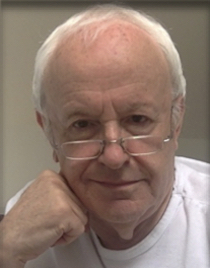
\includegraphics[width=2.19in]{assets/RPF-thumbnail} \caption{This image should really be one that nicely summarises your topic. Not Roger.}\label{fig:mainp}
\end{figure}

\section*{Keynote Lecture}\label{keynote-lecture-6}
\addcontentsline{toc}{section}{Keynote Lecture}

\subsection*{Keynote Speaker Name - Keynote Speaker
Title}\label{keynote-speaker-name---keynote-speaker-title-2}
\addcontentsline{toc}{subsection}{Keynote Speaker Name - Keynote Speaker
Title}

\textbf{Keynote Speaker Affiliation}

\subsection*{About Keynote Speaker}\label{about-keynote-speaker-2}
\addcontentsline{toc}{subsection}{About Keynote Speaker}

\begin{quote}
bio bio bio
\end{quote}

\section*{Practical Session - Practical Session
Title}\label{practical-session---practical-session-title-2}
\addcontentsline{toc}{section}{Practical Session - Practical Session
Title}

\textbf{Led by Practical Session Lead}

\subsection*{Aims and Objectives}\label{aims-and-objectives-6}
\addcontentsline{toc}{subsection}{Aims and Objectives}

\begin{enumerate}
\def\labelenumi{\arabic{enumi}.}
\tightlist
\item
  Teach
\item
  Learn
\item
  Profit
\end{enumerate}

Lorem ipsum dolor sit amet, consectetur adipiscing elit. In iaculis
sagittis metus quis malesuada. Vestibulum laoreet vel tortor at tempor.
Mauris blandit volutpat risus, et placerat odio varius eget. Cras vitae
diam sollicitudin justo vehicula ultrices. Curabitur consequat ornare
odio ac hendrerit. Mauris bibendum diam nec gravida molestie. Nullam
interdum, nulla eget sollicitudin elementum, ante lorem auctor odio, sit
amet varius diam magna et lectus. Sed vehicula velit velit, convallis
mollis erat laoreet nec. Cras semper blandit felis vel iaculis. Sed in
mollis nulla. Nulla sed egestas odio, nec finibus lectus. In vel
porttitor lacus, nec tincidunt neque. Suspendisse at magna non neque
congue fermentum at ut augue. Vivamus suscipit finibus tortor, ut
accumsan dui pretium nec. Integer luctus eros non convallis ornare.

Pellentesque dapibus arcu rutrum neque tempor, ac consequat nisi
consectetur. Nunc eu tortor sed lorem vehicula finibus. Sed sed lacus at
erat fringilla auctor. Aenean malesuada mi est, sit amet molestie ante
malesuada in. Aenean elit risus, imperdiet quis pretium ac, imperdiet a
turpis. Praesent cursus, orci a viverra tincidunt, augue tortor volutpat
erat, a elementum nisi ante vel nisl. Vestibulum purus nisl, imperdiet
egestas ultricies nec, tempor vitae ligula. Integer dapibus magna vitae
orci pharetra rhoncus. Vestibulum in mauris feugiat, pulvinar massa ac,
convallis lacus. In hac habitasse platea dictumst.

\chapter*{Translations and Tipping the
Balance}\label{translations-and-tipping-the-balance}
\addcontentsline{toc}{chapter}{Translations and Tipping the Balance}

\textbf{Led by Matt Moscou and Peter Van Esse}

\emph{Exploiting Knowledge of Plant Pathogen Interactions for Durable
Disease Resistance}

Lorem ipsum dolor sit amet, consectetur adipiscing elit. In iaculis
sagittis metus quis malesuada. Vestibulum laoreet vel tortor at tempor.
Mauris blandit volutpat risus, et placerat odio varius eget. Cras vitae
diam sollicitudin justo vehicula ultrices. Curabitur consequat ornare
odio ac hendrerit. Mauris bibendum diam nec gravida molestie. Nullam
interdum, nulla eget sollicitudin elementum, ante lorem auctor odio, sit
amet varius diam magna et lectus. Sed vehicula velit velit, convallis
mollis erat laoreet nec. Cras semper blandit felis vel iaculis. Sed in
mollis nulla. Nulla sed egestas odio, nec finibus lectus. In vel
porttitor lacus, nec tincidunt neque. Suspendisse at magna non neque
congue fermentum at ut augue. Vivamus suscipit finibus tortor, ut
accumsan dui pretium nec. Integer luctus eros non convallis ornare.

Pellentesque dapibus arcu rutrum neque tempor, ac consequat nisi
consectetur. Nunc eu tortor sed lorem vehicula finibus. Sed sed lacus at
erat fringilla auctor. Aenean malesuada mi est, sit amet molestie ante
malesuada in. Aenean elit risus, imperdiet quis pretium ac, imperdiet a
turpis. Praesent cursus, orci a viverra tincidunt, augue tortor volutpat
erat, a elementum nisi ante vel nisl. Vestibulum purus nisl, imperdiet
egestas ultricies nec, tempor vitae ligula. Integer dapibus magna vitae
orci pharetra rhoncus. Vestibulum in mauris feugiat, pulvinar massa ac,
convallis lacus. In hac habitasse platea dictumst.

Aenean sed leo sit amet dolor congue semper. Curabitur non malesuada
erat. Phasellus scelerisque rutrum tristique. Duis posuere quam tellus,
eu posuere lorem convallis facilisis. Duis euismod tincidunt neque, eu
pellentesque nisi mollis sed. Suspendisse eu nunc rutrum massa iaculis
rhoncus rutrum nec velit. Nulla et erat quis urna malesuada auctor.
Vestibulum sit amet diam maximus, luctus nulla mollis, vestibulum nisi.

\begin{figure}
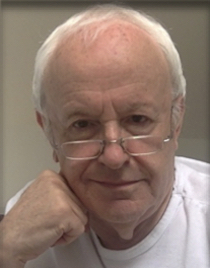
\includegraphics[width=2.19in]{assets/RPF-thumbnail} \caption{This image should really be one that nicely summarises your topic. Not Roger.}\label{fig:maint}
\end{figure}

\section*{Keynote Lecture}\label{keynote-lecture-7}
\addcontentsline{toc}{section}{Keynote Lecture}

\subsection*{Keynote Speaker Name - Keynote Speaker
Title}\label{keynote-speaker-name---keynote-speaker-title-3}
\addcontentsline{toc}{subsection}{Keynote Speaker Name - Keynote Speaker
Title}

\textbf{Keynote Speaker Affiliation}

\subsection*{About Keynote Speaker}\label{about-keynote-speaker-3}
\addcontentsline{toc}{subsection}{About Keynote Speaker}

\begin{quote}
bio bio bio
\end{quote}

\section*{Practical Session - Practical Session
Title}\label{practical-session---practical-session-title-3}
\addcontentsline{toc}{section}{Practical Session - Practical Session
Title}

\textbf{Led by Matt Moscou}

\subsection*{Aims and Objectives}\label{aims-and-objectives-7}
\addcontentsline{toc}{subsection}{Aims and Objectives}

\begin{enumerate}
\def\labelenumi{\arabic{enumi}.}
\tightlist
\item
  Understand different methods for resistance loci
\item
  Introduce basic R packages for QTL analysis
\item
  Understand how to link genotype (genetic maps) with phenotype
  (continuous/discrete measurements) with packages.
\end{enumerate}

Mendelian inheritance of resistance to plant pathogens was first
established by Sir Roland Henry Biffen in 1907. By the end of the 20th
century, the link of phenotype and genotype was established by map-based
cloning of plant resistance genes to a range of plant pathogens.
Although substantial advances have been made in cloning resistance genes
from model species with small genomes, technical hurdles still exist for
large complex genomes that may have little or no sequence information.
This practical will consist of a general introduction of the different
methodologies and approaches for identifying loci contributing to
resistance in complex uncharacterized genomes and a tutorial on using
R/qtl to link genotype (genetic maps) with phenotype (both quantitative
and qualitative data).

\chapter*{General Information}\label{general-information}
\addcontentsline{toc}{chapter}{General Information}

\section*{Arriving into Norwich}\label{arriving-into-norwich}
\addcontentsline{toc}{section}{Arriving into Norwich}

\subsection*{Arriving by Air}\label{arriving-by-air}
\addcontentsline{toc}{subsection}{Arriving by Air}

\textbf{Norwich International Airport}

\href{http://www.norwichairport.co.uk/}{Norwich International Airport}
is served by \href{http://www.klm.com/}{KLM} and the regional carriers
\href{http://www.flybe.com/}{Flybe},
\href{http://www.bmiregional.com/}{BMI Regional}, and
\href{http://www.easternairways.com/}{Eastern Airways}, with direct
connections to Amsterdam, Manchester, Edinburgh, and Aberdeen. Form the
airport you can take a taxi or
\href{http://www.travelineeastanglia.org.uk/ea/XSLT_TTB_REQUEST?language=en\&command=direct\&net=ea\&line=21603\&sup=\%20\&project=y08\&outputFormat=0\&itdLPxx_displayHeader=false\&lineVer=1\&itdLPxx_spTr=1}{local
bus} (with transfer) to get to the Norwich Research Park. Note that if
you fly out of Norwich airport you will need to pay a
\href{http://www.norwichairport.co.uk/content.asp?pid=92}{£10 Airport
Development Fee} before you can go to your gate. Norwich airport is,
however, a very convenient way to reach Norwich from outside the UK.

\textbf{London Airports}

You can also arrive at any of the London airports and take a train or
coach to Norwich. Stansted Airport is the closest and has direct rail
connections to Norwich.

\subsection*{Arriving by Train}\label{arriving-by-train}
\addcontentsline{toc}{subsection}{Arriving by Train}

Another option, especially if you are based in the UK, or are arriving
at another airport, it to take Britain's national train network to
\href{http://www.nationalrail.co.uk/stations_destinations/NRW.aspx}{Norwich
Train Station}, located in downtown Norwich. From there you can take a
local bus or a taxi to Norwich Research Park.
\href{http://www.nationalrail.co.uk/}{National Rail} and
\href{http://www.thetrainline.com/stations/norwich}{TheTrainLine} are
two comprehensive online resource for booking train travel within the
UK.

\subsection*{Arriving by Coach}\label{arriving-by-coach}
\addcontentsline{toc}{subsection}{Arriving by Coach}

You can also arrive in Norwich via coach.
\href{http://www.norfolk.gov.uk/Travel_and_transport/TravelNorfolk/Buses/Bus_interchanges_and_stops/NCC155388}{Norwich
Bus Station} is downtown and is also served by local buses and taxis
once you arrive.

\subsection*{Arriving by Car and
Parking}\label{arriving-by-car-and-parking}
\addcontentsline{toc}{subsection}{Arriving by Car and Parking}

See the \href{http://www.tsl.ac.uk/contact/}{Sainsbury Laboratory} and
\href{https://www.uea.ac.uk/about/visiting-staying/getting-here}{UEA}
\emph{getting here} pages.

Parking at the Conference Centre is
``\href{http://www.venue-norwich.info/FAQs.html}{ample and free for all
events}''. If you require parking at the conference venue, please use
the JIC Visitor's car park (follow the signs we will put up). When you
are at registration, please tell us your license plate number, make, and
colour so we can register it with JIC security.

Those staying at UEA will be able to park in the Main car park on
campus. Parking will be available in the Main car park on campus. UEA
car park charges are listed on the
\href{https://portal.uea.ac.uk/estates/travel-and-transport/by-car/parking-for-visitors}{UEA
car parking for visitors} page

\subsection*{Getting from and into Central Norwich by
Bus}\label{getting-from-and-into-central-norwich-by-bus}
\addcontentsline{toc}{subsection}{Getting from and into Central Norwich
by Bus}

\href{http://www.firstgroup.com/ukbus/suffolk_norfolk/journey_planning/maps/}{First
Group} is the major local bus provider in Norwich.
\href{http://www.firstgroup.com/ukbus/suffolk_norfolk/assets/pdfs/journey_planning/maps/norwich_map.pdf}{This
map shows the complete network}, and these buses specifically serve the
Norwich Research Park or the UEA campus:

\begin{itemize}
\tightlist
\item
  \textbf{\href{https://www.firstgroup.com/norfolk-suffolk/plan-journey/timetables/?operator=22\&service=11/12\&page=1\&redirect=no}{11/12}}:
  Can catch these routes by walking down Colney Lane, towards the
  Hospital, and at the first bus stop past the roundabout.
\item
  \textbf{\href{https://www.firstgroup.com/norfolk-suffolk/plan-journey/timetables/?operator=22\&service=13/13A/13B/13C/X13\&page=1\&redirect=no}{13/13A/13B/13C/X13}}:
  Can catch these routes by walking down Colney Lane, towards the
  Hospital, and at the first bus stop past the roundabout.
\item
  \textbf{\href{https://www.firstgroup.com/norfolk-suffolk/plan-journey/timetables/?operator=22\&service=21\&page=1\&redirect=no}{21/21A/22}}:
  Can catch these right outside Norwich Research Park, on Colney Lane.
\item
  \textbf{\href{https://www.firstgroup.com/norfolk-suffolk/plan-journey/timetables/?operator=22\&service=25\&page=1\&redirect=no}{25}}:
  Goes from the rail station through the UEA campus, all the way to the
  end of Chancellor's Drive.
\item
  \textbf{\href{http://www.firstgroup.com/ukbus/suffolk_norfolk/journey_planning/timetables/index.php?operator=22\&service=26\&page=1\&redirect=no}{26/26A}}:
  Goes from the rail station to University and nearby hospital. Can
  catch the 26 right out Norwich Research Park, on Colney Lane.
\item
  These bus stops have been added to the
  \href{https://drive.google.com/open?id=1z7gP4EFxyaGBmp69A2woREZWNj0\&usp=sharing}{Summer
  School Google Map}.
\end{itemize}

\section*{Checking into Accomodation}\label{checking-into-accomodation}
\addcontentsline{toc}{section}{Checking into Accomodation}

Accommodation will be at the UEA, Britten House. Check in will be at the
UEA Security Lodge at any time from 2pm on the day of your arrival.

\section*{Meals}\label{meals}
\addcontentsline{toc}{section}{Meals}

\subsection*{Breakfast and Lunch}\label{breakfast-and-lunch}
\addcontentsline{toc}{subsection}{Breakfast and Lunch}

Breakfast in the Zest Restaurant is served each day from 8 am to 9 am.
Lunches can be purchased from The Centrum building on site, a range of
salads, sandwiches, soups and hot meals are available. Coffee, tea and
other beverages will be available during breaks.

\subsection*{Evening Meals}\label{evening-meals}
\addcontentsline{toc}{subsection}{Evening Meals}

Evening meals are self catered. The official conference dinner is on
Friday 4th August.

\subsubsection*{Dining Out}\label{dining-out}
\addcontentsline{toc}{subsubsection}{Dining Out}

Norwich is a compact, walkable city with abundant restaurants and cafes.
Head to either Rampant Horse Street area, The Lanes, or the Tombland
area.

UEA Restaurant facilities on campus provide everything from a simple
coffee and sandwich to a full meal at eateries Blend, Zest, Vista, Café
Direct, Cafe 57 and the Sainsbury Centre for Visual Arts Gallery Café,
though these have restricted opening times, usually until 8pm only and
especially outside of terms.

\subsubsection*{Dining In}\label{dining-in}
\addcontentsline{toc}{subsubsection}{Dining In}

The lodging buildings each have a shared kitchen and you will be able to
prepare small meals there. There is a small supermarket on site in the
main plaza, a short walk from the lodging. There are also three
supermarkets just off campus and within walking distance. These are
marked on the included map.

\section*{Getting Around}\label{getting-around}
\addcontentsline{toc}{section}{Getting Around}

Lodging is at The University of East Anglia, in Britten House. Parking
is available in the main campus car park. There is a custom Google Map
with all venues and Norwich Airport and train and bus stations:
\href{https://drive.google.com/open?id=1z7gP4EFxyaGBmp69A2woREZWNj0\&usp=sharing}{Summer
School Map}

\section*{Site Registration}\label{site-registration}
\addcontentsline{toc}{section}{Site Registration}

On the first morning of The Summer School, please go to the John Innes
Centre Reception for 10 am. We can then sign you into the register
on-site and show you to the training rooms.

\section*{Emergency Contacts}\label{emergency-contacts}
\addcontentsline{toc}{section}{Emergency Contacts}

\subsection*{Internal Emergency First
Aid}\label{internal-emergency-first-aid}
\addcontentsline{toc}{subsection}{Internal Emergency First Aid}

Dial \textbf{333}, ask operator for a First Aider or an ambulance. Or
dial \textbf{9 999} for emergency services directly.

\subsection*{Hospital}\label{hospital}
\addcontentsline{toc}{subsection}{Hospital}

The Norfolk and Norwich University Hospital is directly located on the
Norwich Research Park: Colney Lane, Norwich, NR4 7UY. Tel: 01603 286286.

\section*{Transport}\label{transport}
\addcontentsline{toc}{section}{Transport}

\begin{itemize}
\tightlist
\item
  Taxis -- Goldstar Taxis 01603 700700 or ABC Taxis 01603 666333
\item
  Bus - First Group is the major local bus provider in Norwich and these
  buses specifically serve the Norwich Research Park or the UEA campus:
\item
  \textbf{\href{https://www.firstgroup.com/norfolk-suffolk/plan-journey/timetables/?operator=22\&service=11/12\&page=1\&redirect=no}{11/12}}:
  Can catch these routes by walking down Colney Lane, towards the
  Hospital, and at the first bus stop past the roundabout.
\item
  \textbf{\href{https://www.firstgroup.com/norfolk-suffolk/plan-journey/timetables/?operator=22\&service=13/13A/13B/13C/X13\&page=1\&redirect=no}{13/13A/13B/13C/X13}}:
  Can catch these routes by walking down Colney Lane, towards the
  Hospital, and at the first bus stop past the roundabout.
\item
  \textbf{\href{https://www.firstgroup.com/norfolk-suffolk/plan-journey/timetables/?operator=22\&service=21\&page=1\&redirect=no}{21/21A/22}}:
  Can catch these right outside Norwich Research Park, on Colney Lane.
\item
  \textbf{\href{https://www.firstgroup.com/norfolk-suffolk/plan-journey/timetables/?operator=22\&service=25\&page=1\&redirect=no}{25}}:
  Goes from the rail station through the UEA campus, all the way to the
  end of Chancellor's Drive.
\item
  \textbf{\href{http://www.firstgroup.com/ukbus/suffolk_norfolk/journey_planning/timetables/index.php?operator=22\&service=26\&page=1\&redirect=no}{26/26A}}:
  Goes from the rail station to University and nearby hospital. Can
  catch the 26 right out Norwich Research Park, on Colney Lane.
\end{itemize}

These bus stops have been added to the
\href{https://drive.google.com/open?id=1z7gP4EFxyaGBmp69A2woREZWNj0\&usp=sharing}{Summer
School Google Map}.

\section*{Norwich and Norwich Research
Park}\label{norwich-and-norwich-research-park}
\addcontentsline{toc}{section}{Norwich and Norwich Research Park}

At the heart of East Anglia Norwich is a vibrant inviting city. Steeped
in historic charm; The Cathedral, The Castle, the most complete medieval
street pattern in the UK, the largest collection of pre-reformation
churches in Northern Europe and the oldest hotel in the UK are all
situated in Norwich. In medieval times Norwich was the second largest
city in England. Norwich has the largest open-air market in England plus
its own mustard ``Colmans mustard'' and Norwich City Football Club, The
Canaries. In 2012 Norwich became a UNESCO city of literature. Norwich
has a fantastic surrounding countryside including the Broads and Norfolk
coast.

The Norwich Research Park, with six independent partner institutions;
UEA, The John Innes Centre, Earlham Institute, Quadram Institute,
Norfolk and Norwich Hospital and The Sainsbury Laboratory. Norwich
Research Park is ranked fourth in the UK for the number of
internationally recognised scientists. UEA has the second highest
graduate retention rate in the country with almost half of all graduates
living and working locally.

\section*{Wifi Connections}\label{wifi-connections}
\addcontentsline{toc}{section}{Wifi Connections}

Wifi is available throughout the site. If you have EDUROAM available,
please use that. If you don't have EDUROAM, you can get guest wireless
passes from The John Innes Centre Reception.

\section*{Social Media}\label{social-media}
\addcontentsline{toc}{section}{Social Media}

Tweeting and other social media activity are encouraged.
\texttt{\#tslsummerschool}, \texttt{@TheSainsburyLab}

\section*{Map}\label{map}
\addcontentsline{toc}{section}{Map}

A live Google Map with useful sites marked is available
\href{https://drive.google.com/open?id=1z7gP4EFxyaGBmp69A2woREZWNj0\&usp=sharing}{here}

A static version is presented below.

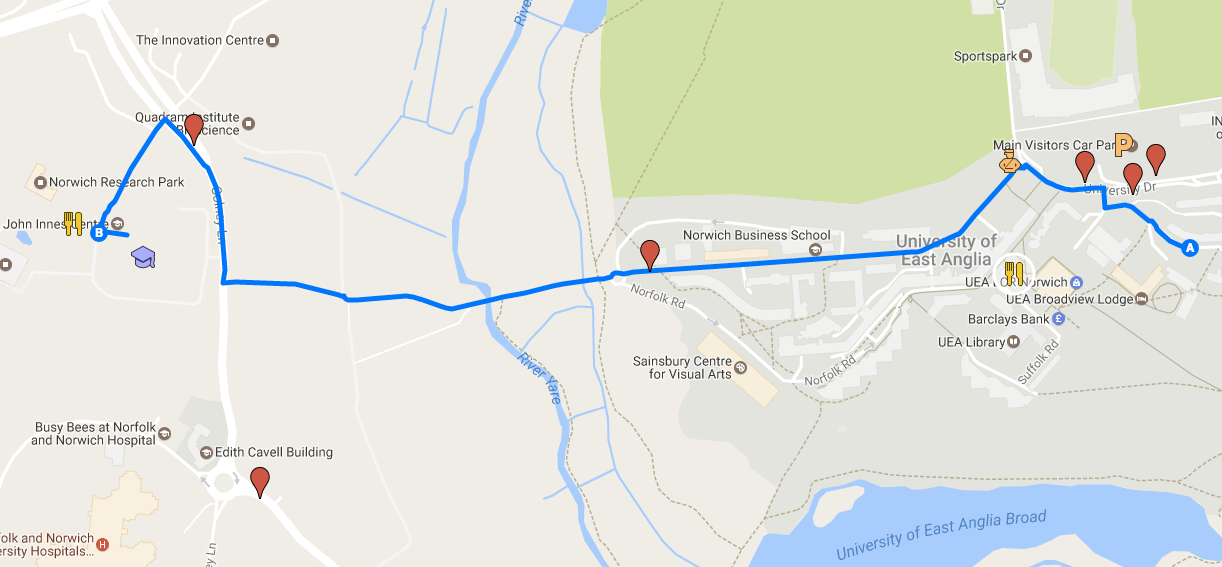
\includegraphics[width=6.11in]{assets/large_map}

\section*{Excursion}\label{excursion}
\addcontentsline{toc}{section}{Excursion}

Sunday is a day of relaxation and we have booked a trip to the north
Norfolk coastal town of Cromer. Perched on the very edge of the north
Norfolk coast, Cromer is famous for its tasty crabs, wide open beaches,
a traditional pier complete with a theatre providing seaside special
variety shows and is awash with small local independent shops. The town
offers a wide choice of restaurants and cafes with not a single coffee
shop chain or national eating or drinking venue to be found. Instead you
have cafes, bars and restaurants owned and operated by local residents
all eager to serve both local residents and visiting guests. The bus
will depart at 1100 am from John Innes Reception.

Later in the day, we have booked a boat in the nearby village of Morston
to take us for a 1 hour trip out on Blakeney Point to see the population
of seals that live there. The boat will leave at 16:45 and the bus will
drop off at Morston from Cromer.

\bibliography{packages.bib,book.bib,res.bib}


\end{document}
